\documentclass[11pt]{article}
\usepackage{algorithm}
\usepackage{algorithmic}
\usepackage{amsmath}
\usepackage{amssymb}
\usepackage{authblk}
\usepackage{bbm}
\usepackage[backend=biber, style=nature]{biblatex}
\usepackage[left=1in, right=1in, top=1in, bottom=1in]{geometry}
\usepackage{graphicx}
\usepackage{float}
\usepackage{multirow}

\usepackage[default]{cantarell}
\usepackage[T1]{fontenc}
\usepackage{sansmath}
% \sansmath  % Makes math use sans-serif
\boldmath  % Makes math bold

\addbibresource{bibliography.bib}

\makeatletter
\renewcommand\AB@affilsepx{\\ \protect\Affilfont} % separate each affiliation with newline
\renewcommand\Authfont{\normalsize\bfseries}      % author name style
\renewcommand\Affilfont{\small\normalfont\itshape\raggedright} % left-align affiliations
\makeatother

\author[1,2]{Daniel Schütte}
\author[2]{Thomas J. Y. Kono}
\author[2,3,*]{Roland F. Schwarz}

\affil[1]{Department I of Internal Medicine, University Hospital Cologne, Cologne, Germany}
\affil[2]{Institute for Computational Cancer Biology (ICCB), Center for Integrated Oncology (CIO), Cancer Research Center Cologne Essen (CCCE), Faculty of Medicine and University Hospital Cologne, University of Cologne, Germany}
\affil[3]{BIFOLD - Berlin Institute for the Foundations of Learning and Data, Berlin, Germany}
\affil[*]{Corresponding author: roland.schwarz@iccb-cologne.org}

\usepackage{fancyhdr}
\pagestyle{fancy}
\fancyhf{}
\fancyhead[L]{\leftmark}
\fancyhead[R]{\thepage}
\renewcommand{\headrulewidth}{0.4pt}

\setlength{\parindent}{0pt}
\setlength{\parskip}{1em}

\title{SC-BIG: A Hierarchical Bayesian Model for Bulk-Informed Single Nucleotide Variant Calling in Single Cells}
\date{Last updated: \today}

\begin{document}

\maketitle

\begin{abstract}
\noindent Single-cell DNA sequencing (scDNA-seq) has emerged as a primary method for investigating cancer genomes and intra-tumor heterogeneity. Despite technological advances, scDNA-seq data suffer from issues arising due to amplification bias and allelic dropout, in addition to the intrinsic error rate of sequencing. Low input DNA quantities further exacerbate these issues. Thus, accurately determining the presence or absence of candidate somatic variants in individual cells remains challenging.

\medskip

\noindent In this work, we develop SC-BIG, a hierarchical Bayesian model that leverages bulk sequencing data from a contemporaneous and representative tumor sample to improve single-cell variant calls. The model propagates uncertainty across multiple biological parameters, such as copy number alterations, sample purity, and variant clonality. The single cell data are used to generate an empirical prior on cancer cell fraction, which cannot be estimated from bulk data alone. The model also estimates technical parameters, such as population-level amplification bias using heterozygous germline single-nucleotide polymorphisms. These biological and technical parameters are used to calculate a matrix of genotype probabilities for all cells.

\medskip

\noindent Across simulated scenarios of varying cancer cell fractions, our method achieves consistently higher classifier performance compared to naive thresholding, with the greatest improvement at high cancer cell fraction. Importantly, the method produces well-calibrated posterior probabilities that provide interpretable uncertainty quantification, enabling direct integration into downstream analyses such as phylogenetic reconstruction. Future work will investigate the model's performance on an existing cohort with paired single-cell and bulk sequencing data and extensions to include other information such as single-cell copy number changes or clonal structure.
\end{abstract}
\newpage

\tableofcontents
\newpage

\section{Introduction}

Single-cell DNA sequencing (scDNA-seq) of cancer samples has enabled characterization of intratumor heterogeneity and clonal dynamics at unprecedented resolution and scale.~\cite{wu2021} Unfortunately, this comes at the cost of increased noise from sparse coverage, amplification errors, and allelic dropout (ADO). Existing bioinformatics methods address these challenges through various strategies. \textit{Monovar}~\cite{zafar2016} discovers SNVs \textit{de novo} using a Bayesian model that incorporates ADO and aggregates evidence across multiple cells.\textit{SCcaller}~\cite{dong2017} and \textit{SCAN-SNV}~\cite{luquette2019} estimate local amplification bias from germline heterozygous SNPs (hSNPs), then apply bias-corrected variant calling.

While these methods enable \textit{de novo} SNV discovery from isolated single-cell experiments, tumor sequencing increasingly comprises multiple data modalities, including scDNA-seq and bulk DNA-seq.~\cite{rozenblatt-rosen2020,leighton2023,chen2025,zhang2023} \textcite{lahnemann2021} were the first to attempt bulk-informed variant calling with \textit{ProSolo}, which genotypes variants in single-cell data using bulk data as a prior. ProSolo builds on the Bayesian framework Varlociraptor~\cite{koester2020} and partitions the joint single-cell and bulk genotype space into seven mutually exclusive events. The latter span three diploid allele frequencies ($\theta_s \in \{0, 0.5, 1\}$) for the single cell and a discretized bulk allele frequency $\theta_b \in [0,1]$. These events capture homozygous reference and alternative genotypes, heterozygosity, allele dropout in both directions, and sequencing errors in both directions. To account for whole-genome amplification artifacts in the single cell, ProSolo incorporates the coverage-dependent beta-binomial model of \textcite{lodato2015}, which was fitted to empirical MDA data and captures allelic imbalance through a mixture of beta-binomial distributions whose shape parameters are linear functions of read depth.

Despite its sophistication, ProSolo makes two strong assumptions that are frequently violated in cancer genomics data. First, all sites are assumed to be diploid: the Lodato model restricts the true single-cell allele frequency to $\theta_s \in \{0, 0.5, 1\}$, preventing it from representing non-diploid copy number states commonly encountered in tumor genomes. Second, all variants are assumed to be clonal ($\text{CCF} = 1$), so that the bulk allele frequency directly reflects the genotype rather than being modulated by subclonal structure. These simplifications can lead to miscalibrated posteriors for subclonal variants at loci with copy number alterations.

Here, we develop SC-BIG, a method to leverage complementary bulk sequencing data to estimate variant presence in individual single cells. Given bulk tumor sequencing, scDNA-seq data, and a set of hSNPs from, for example, an accompanying normal sample, we compute the probability that a specific candidate mutation observed in bulk is present in a certain cell. SC-BIG relaxes both of ProSolo's key assumptions: it supports copy number states $C \in \{1, \ldots, 10\}$ with arbitrary multiplicity $m \leq C$, and it explicitly models subclonal variants by marginalizing over cancer cell fraction. Because CCF suffers from inherent undecidability, a respective prior is estimated from a pseudo-bulk. To simplify the inference algorithm, we assume that all cells are malignant, which can usually be determined through orthogonal data like copy number changes, and focus on variant presence rather than estimating an exact variant allele frequency (VAF). We use simulated data to provide a proof of principle and show that SC-BIG performs favorably compared to both naive VAF thresholding and the ProSolo implementation of \textcite{lahnemann2021}.

\section{Methods}

SC-BIG takes as input bulk and single-cell read counts at a candidate variant site, together with read counts at nearby germline heterozygous SNPs (Figure~\ref{fig:input-data}). The inference proceeds in four steps (Figure~\ref{fig:graphical-abstract}). First, amplification bias is quantified by fitting a beta-binomial model to pooled germline SNP data across all cells. Second, an empirical prior on cancer cell fraction (CCF) is constructed from the aggregate fraction of cells showing variant reads. Third, a CCF posterior is obtained from bulk data by marginalizing over copy number, multiplicity, and tumor purity via MCMC. Fourth, per-cell variant probabilities are computed by combining the CCF posterior with a single-cell likelihood that accounts for amplification bias under one of two error models: a technology-agnostic beta-binomial or the MDA-specific model of \textcite{lodato2015}. Because each cell is scored independently given the shared bulk posterior, inference is fully parallelizable.

\begin{figure}[htbp]
    \centering
    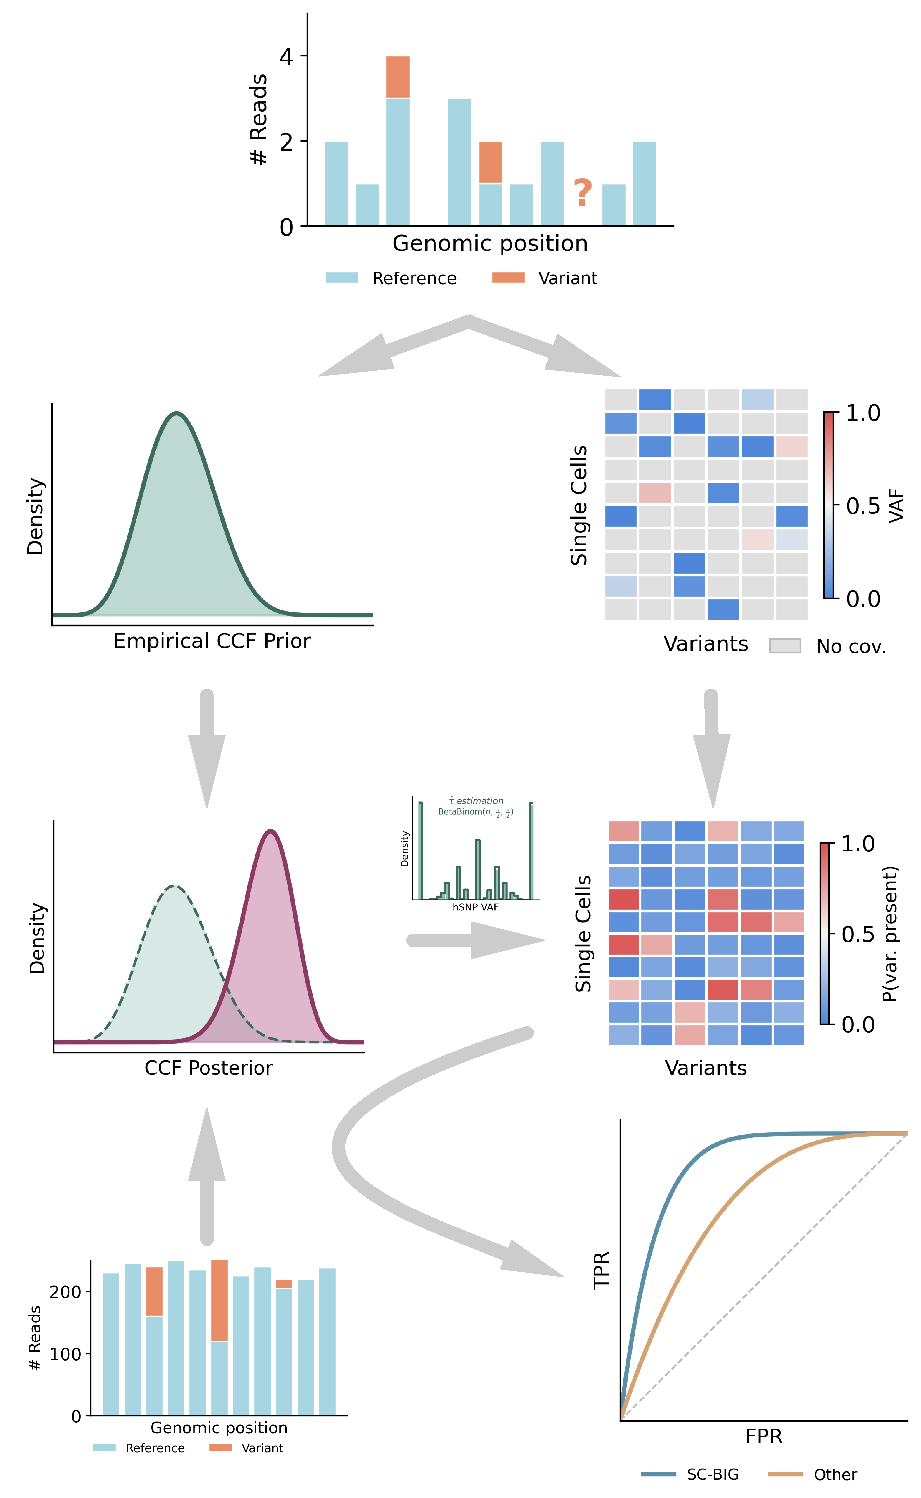
\includegraphics[width=0.75\textwidth]{graphical_abstract/graphical_abstract.pdf}
    \caption{\textbf{SC-BIG method overview.} Starting from sparse single-cell reads at a candidate variant site (top), the method constructs an empirical CCF prior from single-cell aggregates and a VAF matrix across cells and variants (middle row, left and right). Bulk read counts and amplification bias estimated from germline heterozygous SNPs ($\tau$ estimation) are combined with the CCF prior to obtain a CCF posterior via MCMC (bottom left). Per-cell variant probabilities are computed by integrating the CCF posterior with single-cell likelihoods, yielding a probability matrix (middle row, right) and improved classification performance (bottom right, ROC curve).}
    \label{fig:graphical-abstract}
\end{figure}

\subsection{Model Formulation}

\begin{figure}[htbp]
    \centering
    \begin{minipage}{\textwidth}
        \raggedright\textbf{a.}\\[0.5em]
        \centering
        \begin{tabular}{lll}
        \hline
        \textbf{Parameter} & \textbf{Symbol} & \textbf{Description} \\
        \hline
        Purity (mean) & $\bar{\pi}$ & Mean estimate for bulk sample purity \\
        Purity (std) & $\sigma_{\pi}$ & Standard deviation estimate for bulk sample purity \\
        Copy number (mean) & $\bar{C}$ & Mean estimate for copy number at candidate site \\
        Copy number (std) & $\sigma_C$ & Standard deviation estimate for copy number \\
        Bulk variant reads & $k_b$ & Number of reads supporting variant in bulk \\
        Bulk total reads & $n_b$ & Total number of reads at candidate site in bulk \\
        Single-cell variant reads & $k_{sc,i}$ & Variant reads at candidate site in cell $i$ \\
        Single-cell total reads & $n_{sc,i}$ & Total reads at candidate site in cell $i$ \\
        Germline SNPs & $\mathcal{H}$ & Set of heterozygous SNPs $\{(k_{g,j}, n_{g,j})\}$ \\
        & & within reasonable (e.g. $\pm 50$ kb) genomic window \\
        Sequencing error rate & $\epsilon_{sc}$ & Global single-cell sequencing error probability \\
        Bulk concentration & $\kappa$ & Overdispersion parameter for bulk data \\
        \hline
        \end{tabular}
    \end{minipage}

    \vspace{1em}

    \begin{minipage}{\textwidth}
        \raggedright\textbf{b.}\\[0.5em]
        \centering
        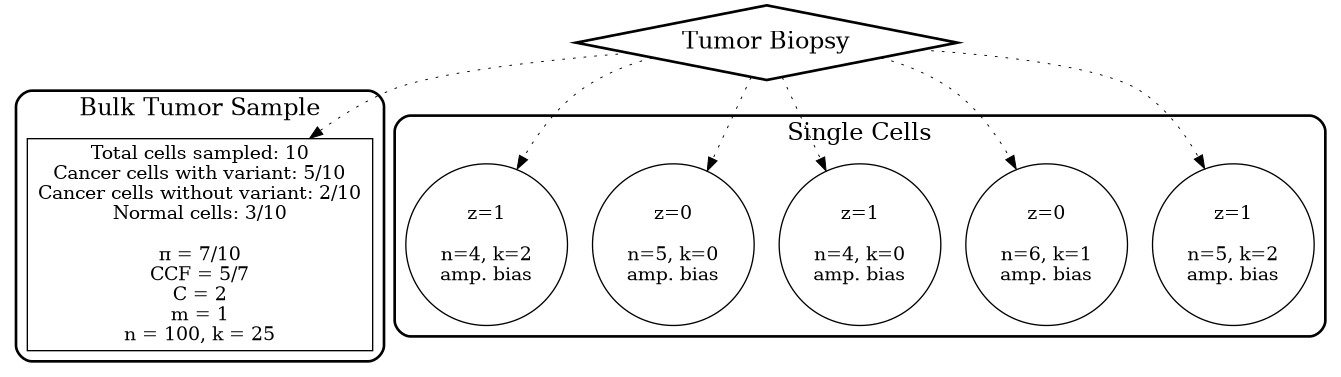
\includegraphics[width=0.9\textwidth]{parameter_illustration.png}
    \end{minipage}

    \caption{\textbf{Model inputs and biological context.} (a) Required input data for SC-BIG. (b) Biological interpretation of model parameters. The bulk tumor contains a mixture of cancer and normal cells, with only a fraction of cancer cells harboring the variant (CCF). Copy number state $C$, purity $\pi$, and variant read counts $k$ are sampled with uncertainty. Germline SNPs $\mathcal{H}$ provide amplification bias estimate.}
    \label{fig:input-data}
\end{figure}

SC-BIG infers the probability that a variant of interest is present in a specific single cell, given bulk evidence. To do so, we let $z \in \{0, 1\}$ indicate variant presence in a single cell:

\begin{equation}
    z =
    \begin{cases}
        1 & \text{if candidate variant is present in single cell} \\
        0 & \text{otherwise}.
    \end{cases}
\end{equation}

The posterior probability of variant presence then is

\begin{equation}
    P(z | D_{sc}, D_{b}) = \frac{
        P(D_{sc} | z, D_{b}) \cdot P(z | D_{b})
    }{
        P(D_{sc} | D_{b})
    }
    ,
\label{eq:base-model-1}
\end{equation}

where the probability depends on both single-cell data $D_{sc}$ and bulk evidence $D_{b}$. For the $z = 1$ case, we assume

\begin{equation}
    P(z=1 | k_{sc}, n_{sc}, D_{b}) = \int_{0}^{1} P(z=1 | k_{sc}, n_{sc}, \text{CCF}) \cdot P(\text{CCF} | D_b)\,d\text{CCF}
    .
\label{eq:hierarchical-marginalization}
\end{equation}

Because cancer cell fraction (CCF) is a latent variable inferred from bulk data, we marginalize over its posterior distribution.
Crucially, $P(z=1 | k_{sc}, n_{sc}, \text{CCF})$ is computed as follows for a given CCF value:

\begin{equation}
    P(z=1 | k_{sc}, n_{sc}, \text{CCF}) = \frac{
        P(k_{sc} | n_{sc}, z=1) \cdot \text{CCF}
    }{
        P(k_{sc} | n_{sc}, z=1) \cdot \text{CCF} + P(k_{sc} | n_{sc}, z=0) \cdot (1-\text{CCF})
    }
    .
\label{eq:posterior-given-ccf}
\end{equation}

The key assumption in equation~\eqref{eq:posterior-given-ccf} is that $P(z=1 | \text{CCF}) = \text{CCF}$, meaning that the probability of a malignant cell harboring the mutation equals the fraction of bulk cancer cells harboring it. Marginalizing over $P(\text{CCF} | D_b)$ in equation~\eqref{eq:hierarchical-marginalization} propagates uncertainty from bulk to single-cell inference.

\begin{figure}[htbp]
    \centering
    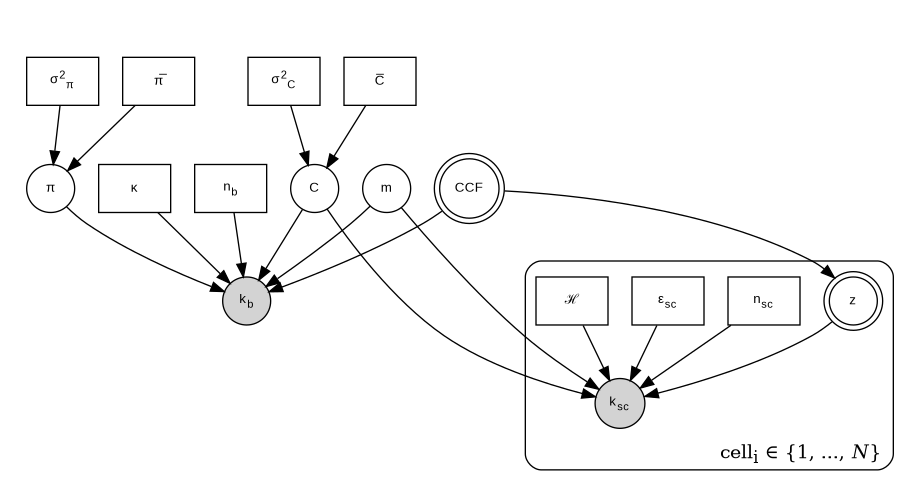
\includegraphics[width=0.9\textwidth]{bayesian_network.png}
    \caption{\textbf{Bayesian network representation of the hierarchical model.} Double circles indicate primary inference targets. Shaded and unshaded circles represent observed and latent random variables, respectively. Rectangles represent fixed input data.}
    \label{fig:bayesian-network}
\end{figure}

Next, the likelihood terms in equation~\eqref{eq:posterior-given-ccf} are defined as:

\begin{equation}
    P(k_{sc} | n_{sc}, z) =
    \begin{cases}
        \text{BetaBinomial}(k_{sc}; n_{sc}, \alpha, \beta) & \text{if } z = 1 \\
        \text{Binomial}(k_{sc}; n_{sc}, \epsilon_{sc}) & \text{if } z = 0.
    \end{cases}
\label{eq:z-likelihood}
\end{equation}

The beta-binomial likelihood for variant-present cells ($z=1$) accounts for amplification bias. Whole-genome amplification introduces stochastic allelic imbalance that causes read counts to deviate from binomial expectations~\cite{dong2017,luquette2019}. This overdispersion manifests as an increased probability of allelic dropout ($k_{sc} \approx 0$) and preferential amplification ($k_{sc} \approx n_{sc}$). We estimate amplification bias from germline heterozygous SNPs (hSNPs), assuming a 1:1 allelic ratio. While this assumption simplifies inference, it might not hold for loci affected by copy number changes. Additionally, we do not investigate genomic windows suitable for the estimation procedure described below, but a method akin to the one described in \textcite{luquette2019} could be used for this purpose in a future version of SC-BIG.

The beta-binomial parameters $\alpha$ and $\beta$ (defined in equation~\eqref{eq:alpha-beta-from-tau} below) are decomposed into two components: a \textit{concentration parameter} $\tau = \alpha + \beta$ that quantifies amplification bias strength, and an \textit{expected VAF} $\alpha/(\alpha+\beta) = m/C$ determined by copy number $C$ and multiplicity $m$. This parameterization preserves the biologically expected mean VAF while capturing overdispersion---low $\tau$ indicates high amplification bias with greater variance around the expected VAF, including dropout events, whereas high $\tau$ approaches binomial behavior.

We estimate a population-level $\tau$ from germline heterozygous SNPs pooled across all cells. Since hSNPs have known 1:1 allelic ratio in diploid regions, their observed VAF variance directly reflects amplification bias. We fit a symmetric beta-binomial ($\alpha = \beta = \tau/2$, expected VAF = 0.5) via maximum likelihood to the pooled data, yielding a single $\tau$ used for all cells. Such a population estimate is more robust compared to using per-cell observations and yields good downstream performance in our simulations.

Given $\tau$, we parameterize the somatic variant beta-binomial as:

\begin{equation}
    \alpha = \tau \cdot \frac{m}{C}
    , \quad
    \beta = \tau \cdot \left(1 - \frac{m}{C}\right)
    ,
\label{eq:alpha-beta-from-tau}
\end{equation}
ensuring mean VAF = $m/C$ while $\tau$ captures population-level overdispersion.

As an alternative to the beta-binomial error model described above, SC-BIG supports the coverage-dependent amplification bias model of \textcite{lodato2015}, which was developed for MDA-amplified single cells and is used by ProSolo.~\cite{lahnemann2021} This model captures allelic imbalance through mixture beta-binomial distributions whose shape parameters are linear functions of read depth, fitted to empirical MDA data.

Since the Lodato model is defined only for diploid allele frequencies $\theta_s \in \{0, 0.5, 1\}$, we map the true allele frequency $m/C$ to the nearest supported value:
\begin{equation}
    \theta_s = \begin{cases}
        0   & \text{if } m/C \leq 0.25 \\
        0.5 & \text{if } 0.25 < m/C \leq 0.75 \\
        1   & \text{if } m/C > 0.75.
    \end{cases}
\label{eq:lodato-af-mapping}
\end{equation}

For each $\theta_s$, the model specifies a distribution over a distorted allele frequency $\rho_s$ via coverage-dependent beta-binomial parameters, and the per-read likelihood is evaluated at $\rho_s$ using a binomial model with base error rate $e$:

\begin{equation}
    P(k_{sc} | n_{sc}, z=1) = \sum_{k_s=0}^{n_{sc}^*}
        P_{\text{read}}(k_{sc} | n_{sc}, \rho_s = k_s / n_{sc}^*)
        \cdot P_{\text{Lodato}}(k_s | n_{sc}^*, \theta_s)
    ,
\label{eq:lodato-likelihood}
\end{equation}

where $n_{sc}^* = \min(n_{sc}, 100)$ is the coverage cap used in the original model, $P_{\text{Lodato}}$ is the Lodato beta-binomial PMF, and $P_{\text{read}}$ is the per-read likelihood:

\begin{equation}
    P_{\text{read}}(k | n, \rho) = \binom{n}{k} \left[\rho(1-e) + (1-\rho)\frac{e}{3}\right]^k \left[(1-\rho)(1-e) + \rho\frac{e}{3}\right]^{n-k}
    .
\end{equation}

At the heterozygous allele frequency ($\theta_s = 0.5$), the Lodato model uses a mixture of two symmetric beta-binomial distributions to capture the bimodal read count distribution characteristic of MDA. At homozygous frequencies ($\theta_s \in \{0, 1\}$), a single beta-binomial with asymmetric parameters models the dropout and error behavior. All parameters are linear functions of coverage, fitted from the empirical data of \textcite{lodato2015} and taken with full precision from the \texttt{libprosic} v0.7.3 source code.

This Lodato error model is well-characterized for MDA-amplified data and enables direct comparison with ProSolo under identical per-read error modeling. However, even when SC-BIG adopts the same Lodato likelihood, several structural differences remain between the two methods. First, SC-BIG marginalizes over a cancer cell fraction posterior inferred from bulk data (equation~\eqref{eq:hierarchical-marginalization}), whereas ProSolo assumes all variants are clonal ($\text{CCF} = 1$) and does not model subclonal structure. Second, SC-BIG supports non-diploid copy number states $C \in \{1, \ldots, 10\}$ with arbitrary multiplicity $m \leq C$; the Lodato allele frequencies are obtained by mapping $m/C$ to the nearest value in $\{0, 0.5, 1\}$ (equation~\eqref{eq:lodato-af-mapping}), preserving the empirically fitted per-read model while permitting copy number variation that ProSolo's strictly diploid framework cannot represent. Third, SC-BIG constructs an empirical CCF prior from single-cell aggregates (equation~\eqref{eq:ccf-prior}), providing an independent source of information absent from ProSolo. Fourth, SC-BIG jointly marginalizes over tumor purity $\pi$ and a geometric multiplicity prior $P(m|C) \propto 2^{-m}$, both of which modulate the expected bulk VAF and thus the CCF posterior; ProSolo uses a flat prior over its seven genotype events and does not model purity. These differences mean that, despite sharing the same per-read error model, SC-BIG and ProSolo can produce substantially different posteriors---particularly for subclonal variants at loci with copy number alterations.

The beta-binomial model of equation~\eqref{eq:alpha-beta-from-tau}, which makes no amplification-technology-specific assumptions, serves as a fall-back for scDNA-seq technologies where the amplification process is less well studied than MDA, such as PTA or DLP+.

To compute equation~\eqref{eq:hierarchical-marginalization}, we need the CCF posterior $P(\text{CCF} | D_b)$. Bulk sequencing provides evidence about population-level CCF, but uncertainty in variant multiplicity $m$ potentially creates a multimodal posterior. For example, a bulk VAF of 0.4 is consistent with both $m=1, \text{CCF} \approx 0.8$ (heterozygous variant in 80\% of cells) and $m=2, \text{CCF} \approx 0.4$ (homozygous variant in 40\% of cells). This multiplicity ambiguity substantially affects individual cell posteriors, particularly for dropout events where different multiplicity assumptions yield different likelihood values.

The expected bulk variant allele frequency depends on purity $\pi$, copy number $C$, multiplicity $m$, and CCF~\cite{tarabichi2021}:
\begin{equation}
    \text{VAF}_{\text{exp}} = \frac{
        \pi \cdot \text{CCF} \cdot m
    }{
        \pi \cdot C + 2 (1-\pi)
    }
    .
\end{equation}

The bulk likelihood is modeled as:
\begin{equation}
    P(k_b | n_b, \text{CCF}, m, \pi, C) = \text{BetaBinomial}(k_b; n_b, \alpha, \beta)
    ,
\end{equation}
with $\alpha = \kappa \cdot \text{VAF}_{\text{exp}}$, $\beta = \kappa \cdot (1-\text{VAF}_{\text{exp}})$, and $\kappa$ being a concentration parameter for bulk overdispersion.

We place priors on the latent parameters. For copy number:
\begin{equation}
    P(C) = \frac{
        \exp\left(-\frac{(C - \bar{C})^2}{2\sigma_C^2}\right)
    }{
    \sum_{j=1}^{10}{\exp\left(-\frac{(j - \bar{C})^2}{2\sigma_C^2}\right)}
    }, \quad C \in \{1, 2, \ldots, 10\}
\end{equation}
(a truncated discrete normal). For purity:
\begin{equation}
    P(\pi) = \mathcal{N}(\pi; \bar{\pi}, \sigma_{\pi}), \quad \pi \in [0.01, 0.99]
    ,
\end{equation}
where values are clamped to $[0.01, 0.99]$ for numerical stability. For multiplicity:
\begin{equation}
    P(m | C) = \begin{cases}
        \frac{1}{C} & \text{(uniform prior)} \\
        \frac{2^{-m}}{\sum_{l=1}^{C} 2^{-l}} & \text{(geometric prior)}
    \end{cases}, \quad m \in \{1, 2, \ldots, C\}
\end{equation}

The geometric prior $P(m|C) \propto 2^{-m}$ favors lower multiplicities, reflecting the expectation that most somatic variants are heterozygous ($m=1$). For $C=2$, this assigns $P(m=1|C=2) = 2/3$ and $P(m=2|C=2) = 1/3$. The geometric prior is used by default.

The CCF posterior is obtained by marginalizing over $\pi$, $C$, and $m$:

\begin{equation}
\begin{gathered}[t]
    P(\text{CCF} | k_b, n_b) = \\
    \frac{
        \sum_m{
            \sum_C{
                \int_{0}^{1}{
                    P(k_b | n_b, \text{CCF}, m, \pi, C) \cdot P(\text{CCF}) \cdot P(m|C) \cdot P(\pi) \cdot P(C) \, d\pi
                }
            }
        }
    }{
        \int_{0}^{1}{
            \sum_m{
                \sum_C{
                    \int_{0}^{1}{
                        P(k_b | n_b, \text{CCF}, m, \pi, C) \cdot P(\text{CCF}) \cdot P(m|C) \cdot P(\pi) \cdot P(C) \, d\pi \,d\text{CCF}
                    }
                }
            }
        }
    }
    .
\end{gathered}
\label{eq:ccf-posterior}
\end{equation}

In practice, we approximate these integrals using hybrid MCMC: for each discrete $(C, m)$ combination, we sample continuous parameters $(\text{CCF}, \pi)$ from the conditional posterior using NUTS (No-U-Turn Sampler)~\cite{hoffman2011}. Each MCMC sample receives a weight proportional to $P(C) \cdot P(m|C) \cdot P(k_b | n_b, \text{CCF}, \pi, C, m)$, ensuring parameter combinations that better explain bulk data receive higher weight. The hierarchical marginalization is computed as a weighted average over posterior samples.

The CCF prior $P(\text{CCF})$ in equation~\eqref{eq:ccf-posterior} can be set to uniform, but we can leverage single-cell aggregate statistics to obtain an informative prior. While individual cells have sparse coverage, the \textit{aggregate fraction} of cells showing variant reads provides evidence about population-level CCF independent of multiplicity.

We model the CCF prior as a Beta distribution conjugate to the binomial likelihood of single-cell observations:
\begin{equation}
    P(\text{CCF}) = \text{Beta}(\text{CCF} \mid k_{\text{pos}} + 1, \, n_{\text{elig}} - k_{\text{pos}} + 1)
    ,
\label{eq:ccf-prior}
\end{equation}
where $k_{\text{pos}}$ is the number of cells with at least one variant read ($k_{sc} \geq 1$) and $n_{\text{elig}}$ is the total number of cells with sufficient coverage ($n_{sc} \geq 3$).

This formulation provides natural regularization. In the limit of sparse or missing single-cell data ($n_{\text{elig}} \to 0$), the prior converges to $\text{Beta}(1, 1)$, equivalent to a uniform prior over $[0, 1]$, ensuring that inference is driven solely by bulk likelihoods when single-cell evidence is weak. As single-cell coverage increases, the prior tightens around the observed cellular prevalence, guiding the resolution of multiplicity ambiguities without imposing hard constraints.

Because single-cell genotyping suffers from allelic dropout, this empirical prior is conservative: it may underestimate CCF when dropout leads to under-counting of variant-positive cells. We believe this conservative behavior is acceptable because the bulk data provides complementary evidence that can correct for dropout-induced bias during posterior inference.

\subsection{Algorithm Summaries}

Algorithm~\ref{alg:inference} summarizes the complete inference procedure.

\begin{algorithm}[htbp]
\caption{Hierarchical Bayesian Inference}
\label{alg:inference}
\begin{algorithmic}[1]
\REQUIRE Bulk data $(k_b, n_b)$, single-cell data $\{(k_{sc,i}, n_{sc,i}, \mathcal{H}_i)\}$, priors $(\bar{\pi}, \sigma_\pi, \bar{C}, \sigma_C)$
\ENSURE $P(z=1 | k_{sc}, n_{sc}, D_b)$ for each cell

\STATE \textbf{Step 1: Estimate population $\tau$} from pooled germline SNPs via MLE (beta-binomial model only)

\STATE \textbf{Step 2: Estimate CCF prior} from single-cell aggregate data
\STATE $n_{\text{elig}} \gets |\{i : n_{sc,i} \geq 3\}|$; \quad $k_{\text{pos}} \gets |\{i : n_{sc,i} \geq 3 \land k_{sc,i} \geq 1\}|$
\STATE Set Beta prior: $\alpha_{\text{CCF}} = k_{\text{pos}} + 1$, $\beta_{\text{CCF}} = (n_{\text{elig}} - k_{\text{pos}}) + 1$

\STATE \textbf{Step 3: Sample CCF posterior} via MCMC with discrete enumeration
\FOR{each $(C, m)$ pair with non-negligible prior}
    \STATE Run NUTS for $(\text{CCF}, \pi)$ conditioned on $(C, m)$
    \STATE Weight samples by $P(C) \cdot P(m|C) \cdot P(k_b | n_b, \text{CCF}, \pi, C, m)$
\ENDFOR

\STATE \textbf{Step 4: Compute single-cell posteriors}
\FOR{each weighted sample $(\text{CCF}, \pi, C, m, w)$}
    \IF{error model is beta-binomial}
        \STATE $L_{z=1} = \text{BetaBinom}(k_{sc}; n_{sc}, \tau m/C, \tau(1-m/C))$
    \ELSIF{error model is Lodato}
        \STATE Map $\theta_s$ from $m/C$ via eq.~\eqref{eq:lodato-af-mapping}; $L_{z=1}$ via eq.~\eqref{eq:lodato-likelihood}
    \ENDIF
    \STATE $L_{z=0} = \text{Binom}(k_{sc}; n_{sc}, \epsilon_{sc})$
    \STATE $P(z=1|\text{sample}) = \frac{\text{CCF} \cdot L_{z=1}}{\text{CCF} \cdot L_{z=1} + (1-\text{CCF}) \cdot L_{z=0}}$
\ENDFOR
\RETURN Weighted average of $P(z=1|\text{sample})$ across all samples
\end{algorithmic}
\end{algorithm}

Lastly, algorithm~\ref{alg:simulation} is used to generate synthetic data for validation. To produce a realistic distribution of cellular prevalences, we use the Kingman coalescent~\cite{wu2021}: starting from $N$ leaf nodes (cells), pairs of lineages are merged backwards in time with coalescence times drawn from $\text{Exp}\binom{n}{2}/N_e$, where $n$ is the current number of lineages and $N_e$ is the effective population size. $M$ somatic mutations are placed on branches proportional to branch length, so that mutations near the root are carried by many cells (high CCF) and mutations near the leaves by few (low CCF). Copy number $C_j \in \{1, 2, 3\}$ at each locus is drawn from a categorical distribution and multiplicity is sampled from a geometric prior $P(m_j | C_j) \propto 2^{-m_j}$, $m_j \in \{1, \ldots, C_j\}$, consistent with the inference model. Branches yielding $\text{CCF} < 0.05$ are redrawn to avoid degenerate cases where sparse single-cell coverage is uninformative. We assume the infinite sites model as well as independence between loci.

Additionally, for each mutation, bulk reads are drawn from a beta-binomial with the expected VAF and single-cell reads are drawn depending on the chosen error model. With the beta-binomial model, cell-specific amplification bias $\tau_i \sim \text{Gamma}(\mu_\tau, \text{CV}_\tau)$ determines overdispersion for both germline SNPs and somatic variants, ensuring that bias estimated from hSNPs transfers to variant calls. With the Lodato model, single-cell reads are sampled from the coverage-dependent beta-binomial PMF (equation~\eqref{eq:lodato-likelihood}) at the mapped allele frequency $\theta_s$ (equation~\eqref{eq:lodato-af-mapping}). Each mutation produces an independent dataset, enabling parallelized inference.

\begin{algorithm}[htbp]
\caption{Coalescent Simulation}
\label{alg:simulation}
\begin{algorithmic}[1]
\REQUIRE $N$ cells, $M$ mutations, $N_e$, purity $\pi$, coverage $(n_b, n_{sc})$, bias $(\mu_\tau, \text{CV}_\tau)$, error model $\in \{\text{beta-binomial}, \text{Lodato}\}$
\ENSURE $M$ independent datasets with bulk and single-cell data

\STATE Generate Kingman coalescent tree with $N$ leaves and $N_e$; assign stem branch $t_{\text{stem}} \sim \text{Exp}(N_e)$ to the root
\FOR{$j = 1$ to $M$}
    \REPEAT
        \STATE Sample branch proportional to length; carriers $\gets$ leaf descendants; $\text{CCF}_j \gets |\text{carriers}|/N$
        \STATE Sample $C_j \in \{1, 2, 3\}$, $m_j \sim \text{Geometric}\{1, \ldots, C_j\}$ with $P(m|C) \propto 2^{-m}$
    \UNTIL{$\text{CCF}_j \geq 0.05$}
    \STATE $k_b \sim \text{BetaBinom}(n_b,\; \kappa \cdot \text{VAF}_b,\; \kappa(1-\text{VAF}_b))$ where $\text{VAF}_b = \pi \cdot \text{CCF}_j \cdot m_j / (\pi C_j + 2(1-\pi))$
    \FOR{$i = 1$ to $N$}
        \STATE $z_i \gets \mathbf{1}[i \in \text{carriers}]$; \quad $\tau_i \sim \text{Gamma}(\mu_\tau, \text{CV}_\tau)$; \quad $n_{sc,i} \sim \text{Poisson}(n_{sc})$
        \IF{$z_i = 1$ \AND beta-binomial model}
            \STATE $k_{sc,i} \sim \text{BetaBinom}(n_{sc,i},\; \tau_i m_j/C_j,\; \tau_i(1-m_j/C_j))$
        \ELSIF{$z_i = 1$ \AND Lodato model}
            \STATE Map $\theta_s$ from $m_j/C_j$ via eq.~\eqref{eq:lodato-af-mapping}; $k_{sc,i} \sim P_{\text{Lodato}}(n_{sc,i}, \theta_s)$
        \ELSE
            \STATE $k_{sc,i} \sim \text{Binom}(n_{sc,i}, \epsilon_{sc})$
        \ENDIF
        \STATE Generate $|\mathcal{H}|$ germline SNPs: $k_{g,l} \sim \text{BetaBinom}(n_{g,l}, \tau_i/2, \tau_i/2)$
    \ENDFOR
\ENDFOR
\RETURN $\{(k_{b,j}, \{k_{sc,i}, n_{sc,i}, \mathcal{H}_i, z_i\}_{i=1}^N, C_j, m_j, \text{CCF}_j)\}_{j=1}^M$
\end{algorithmic}
\end{algorithm}

\subsection{Implementation \& Evaluation}

The model is implemented as a Python package providing both a library API and command-line interface. The interface provides subcommands for simulation (\texttt{simulate}, \texttt{simulate-tree}), inference (\texttt{infer}, \texttt{infer-prosolo}), and method comparison (\texttt{compare}). All simulation hyperparameters (CCF, purity, copy number, coverage, error rates, amplification bias parameters) and inference settings (prior distributions, number of MCMC samples, decision threshold) are configurable via command-line arguments.

Bayesian inference uses Pyro~\cite{bingham2019}, a probabilistic programming library built on PyTorch. Pyro enables direct specification of the hierarchical model structure and provides a NUTS (No-U-Turn Sampler) implementation~\cite{hoffman2011} for gradient-based sampling of continuous parameters (CCF, purity). Discrete parameters (copy number, multiplicity) are handled via enumeration, with likelihood-weighted combination of posterior samples across discrete states. Single-cell inference is parallelizable across cells since each posterior probability is computed independently given bulk data, enabling efficient multi-core execution.

For comparison with ProSolo, the \texttt{infer-prosolo} subcommand generates synthetic BAM files from the simulated read counts using \texttt{pysam} and invokes the ProSolo v0.6.1 binary as a subprocess. For each cell at each mutation site, a minimal reference FASTA, candidate VCF, bulk BAM, and single-cell BAM are created, with base qualities set to the Phred score corresponding to the simulated error rate ($Q = -10\log_{10}(e)$). The seven PHRED-scaled event posteriors emitted by ProSolo are converted to linear probabilities, and $P(\text{alt present})$ is computed as the union over the five alt-present events (HET, HOM\_ALT, ADO\_TO\_REF, ADO\_TO\_ALT, ERR\_REF), following equation~9 of \textcite{lahnemann2021}.

SC-BIG is available as an open-source package at \url{https://bitbucket.org/schwarzlab/tool-sc-big} under the GNU General Public License v3.

We evaluate classification performance using two complementary metrics. F1-score balances precision and recall through their harmonic mean:

\begin{equation}
    \text{F1} = \frac{2 \cdot \text{TP}}{2 \cdot \text{TP} + \text{FP} + \text{FN}}
    ,
\end{equation}

where TP, FP, and FN denote true positives, false positives, and false negatives respectively. We compute F1 across all decision thresholds and report the maximum achievable value with its corresponding optimal threshold. ROC-AUC (area under the receiver operating characteristic curve) measures discrimination ability independent of threshold choice:

\begin{equation}
    \text{ROC-AUC} = \int_0^1 \text{TPR}(\text{FPR}^{-1}(t)) \, dt
    ,
\end{equation}

where TPR (true positive rate) $= \text{TP}/(\text{TP}+\text{FN})$ and FPR (false positive rate) $= \text{FP}/(\text{FP}+\text{TN})$. ROC-AUC equals the probability that a randomly chosen positive instance receives a higher score than a randomly chosen negative instance.

\section{Results}

We evaluate SC-BIG on three CCF scenarios (Table~\ref{tab:scenario-parameters}): high ($\text{CCF}=0.8$), intermediate ($\text{CCF}=0.5$), and low ($\text{CCF}=0.2$) cellular prevalences. All other parameters are fixed to be diploid ($C=2$), heterozygous ($m=1$), pure tumor ($\pi=1.0$), sparse coverage ($\bar{n}_{sc}=3$).

\begin{table}[htbp]
\centering
\begin{tabular}{llcl}
\hline
\textbf{Parameter} & \textbf{Symbol} & \textbf{Value} \\
\hline
\multicolumn{3}{l}{\textit{Variable parameter}} \\
Cancer Cell Fraction & CCF & 0.2, 0.5, 0.8 \\
\hline
\multicolumn{3}{l}{\textit{Fixed biological parameters}} \\
Tumor Purity & $\pi$ & 1.0 \\
Copy Number & $C$ & 2 \\
Multiplicity & $m$ & 1 \\
\hline
\multicolumn{3}{l}{\textit{Fixed sequencing parameters}} \\
Single-Cell Coverage & $\bar{n}_{sc}$ & 3 \\
Bulk Coverage & $n_b$ & 250 \\
Sequencing Error Rate & $\epsilon_{sc}$ & 0.02 \\
Germline SNPs & $|\mathcal{H}|$ & 600 \\
Bulk Concentration & $\kappa$ & 100 \\
\hline
\multicolumn{3}{l}{\textit{Fixed amplification bias parameters}} \\
Concentration Mean & $\mu_\tau$ & 80 \\
Concentration CV & $\text{CV}_\tau$ & 0.05 \\
\hline
\multicolumn{3}{l}{\textit{Simulation settings}} \\
Number of Cells & $N$ & 500 \\
Random Seed & -- & 42 \\
\hline
\multicolumn{3}{l}{\textit{Inference prior parameters}} \\
Purity Prior & $\pi \sim \mathcal{N}(\mu, \sigma)$ & (1.0, 0.01) \\
Copy Number Prior & $C \sim \mathcal{N}(\mu, \sigma)$ & (2.0, 0.3) \\
Multiplicity Prior & $P(m|C)$ & geometric \\
\hline
\end{tabular}
\caption{Simulation and inference parameters for the three CCF scenarios}
\label{tab:scenario-parameters}
\end{table}

For each scenario, we compare SC-BIG to a ``naive'' caller that scores each cell by its observed VAF ($k_{sc}/n_{sc}$) and applies a threshold. Both methods are evaluated using F1-score (across all thresholds) and ROC-AUC.

\subsection{High Prevalence Scenario}

Figure~\ref{fig:high-ccf-results} shows results for the high CCF scenario. The posterior versus $k_{sc}$ plot (Figure~\ref{fig:high-ccf-results}a) shows a systematic shift of variant-present cell posteriors toward higher values at every $k_{sc}$ level, including $k_{sc}=0$ (complete dropout) where both populations present with identical read evidence. The Bayesian method achieves maximum F1 = 0.94 at threshold 0.32, compared to F1 = 0.91 for naive thresholding (Figure~\ref{fig:high-ccf-results}b). ROC-AUC is 0.934 for Bayesian versus 0.857 for naive (Figure~\ref{fig:high-ccf-results}c).

\begin{figure}[htbp]
    \centering
    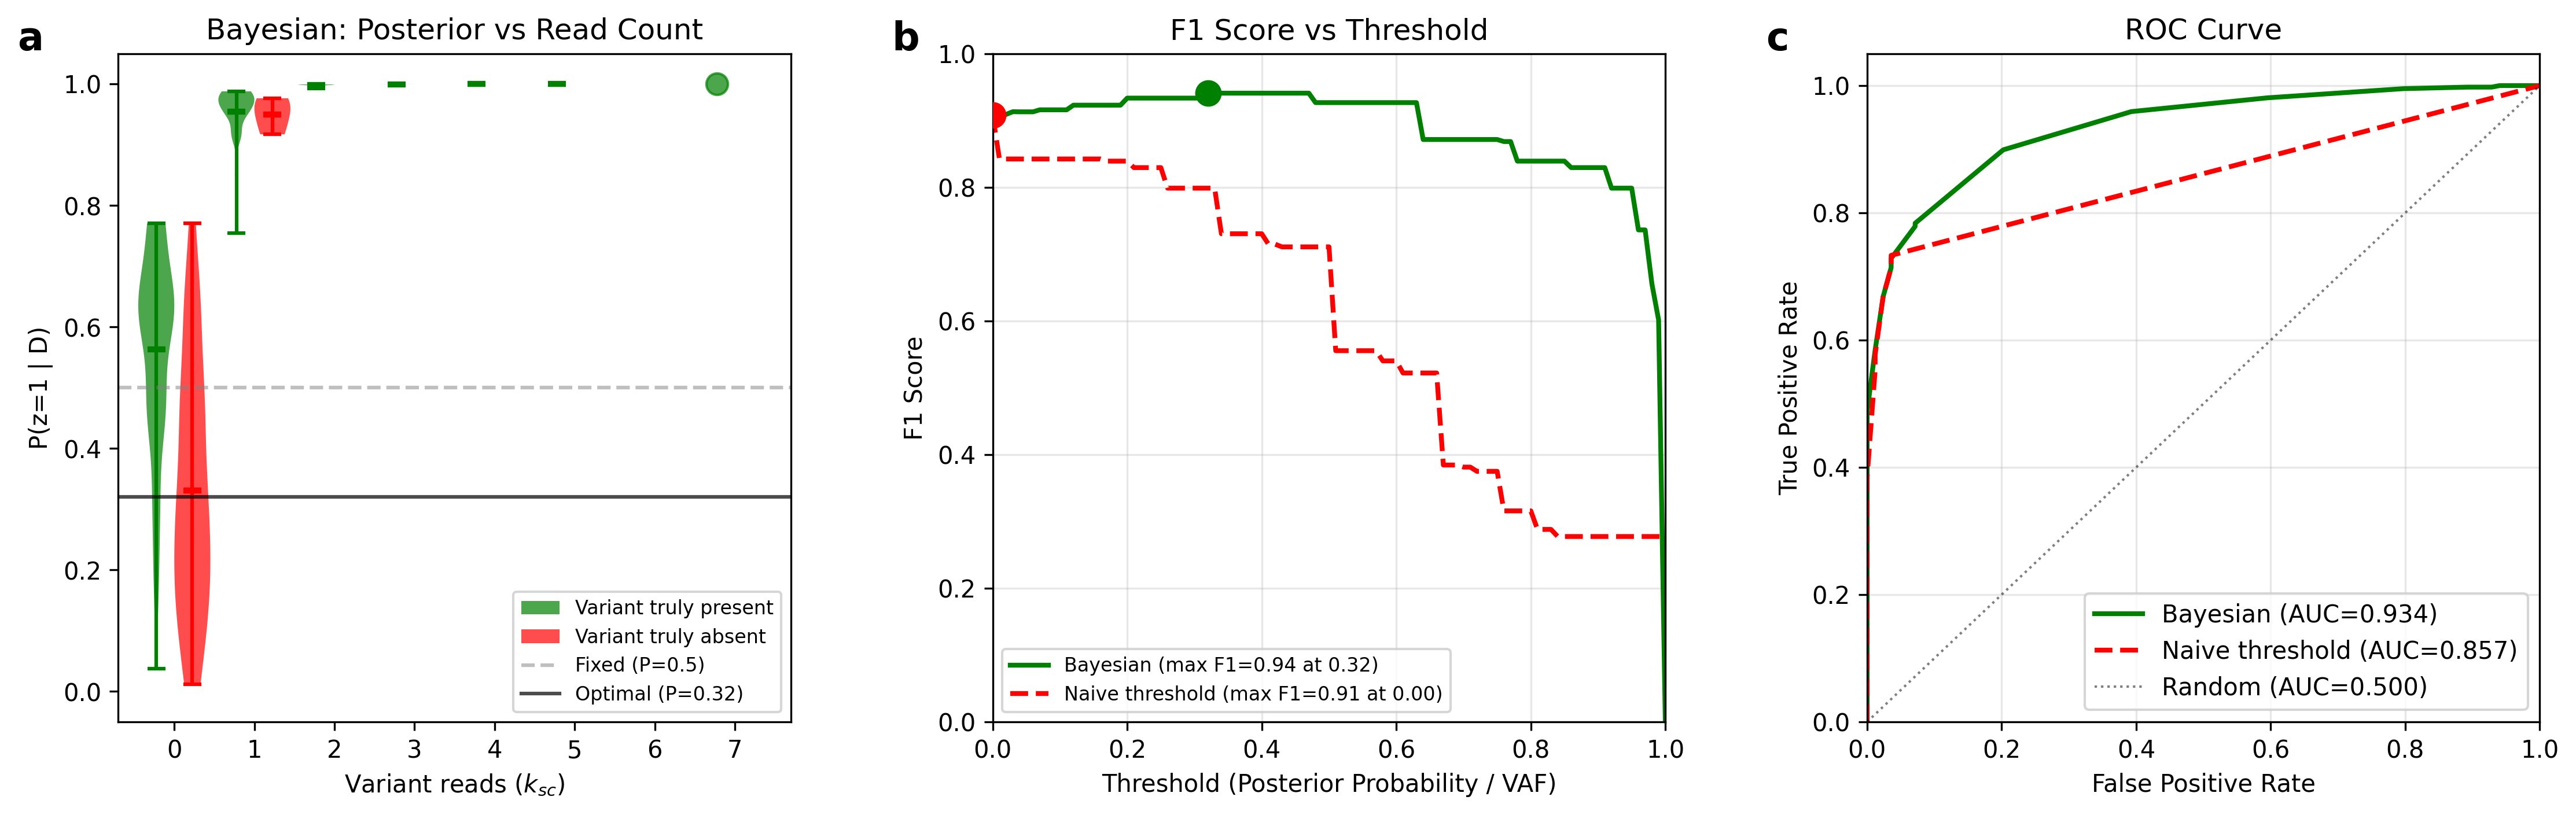
\includegraphics[width=\textwidth]{../data/almost_all_cells_positive/bayesian_plots.png}
    \caption{\textbf{High CCF inference results (CCF = 0.8).} (a) Posterior probability versus variant read count $k_{sc}$. Violin plots show the distribution of posteriors for variant-present cells (green) and variant-absent cells (red) at each $k_{sc}$ value; single points indicate $k_{sc}$ values with only one observation. (b) F1-score as a function of decision threshold for Bayesian (green) and naive (red) methods. (c) ROC curves showing Bayesian versus naive AUC.}
    \label{fig:high-ccf-results}
\end{figure}

The CCF posterior (Figure~\ref{fig:high-ccf-diagnostics}a) accurately recovers the true value, with mean 0.771 versus the simulation parameter of 0.80. Calibration analysis (Figure~\ref{fig:high-ccf-diagnostics}c) demonstrates well-calibrated posteriors across the full probability range.

\begin{figure}[htbp]
    \centering
    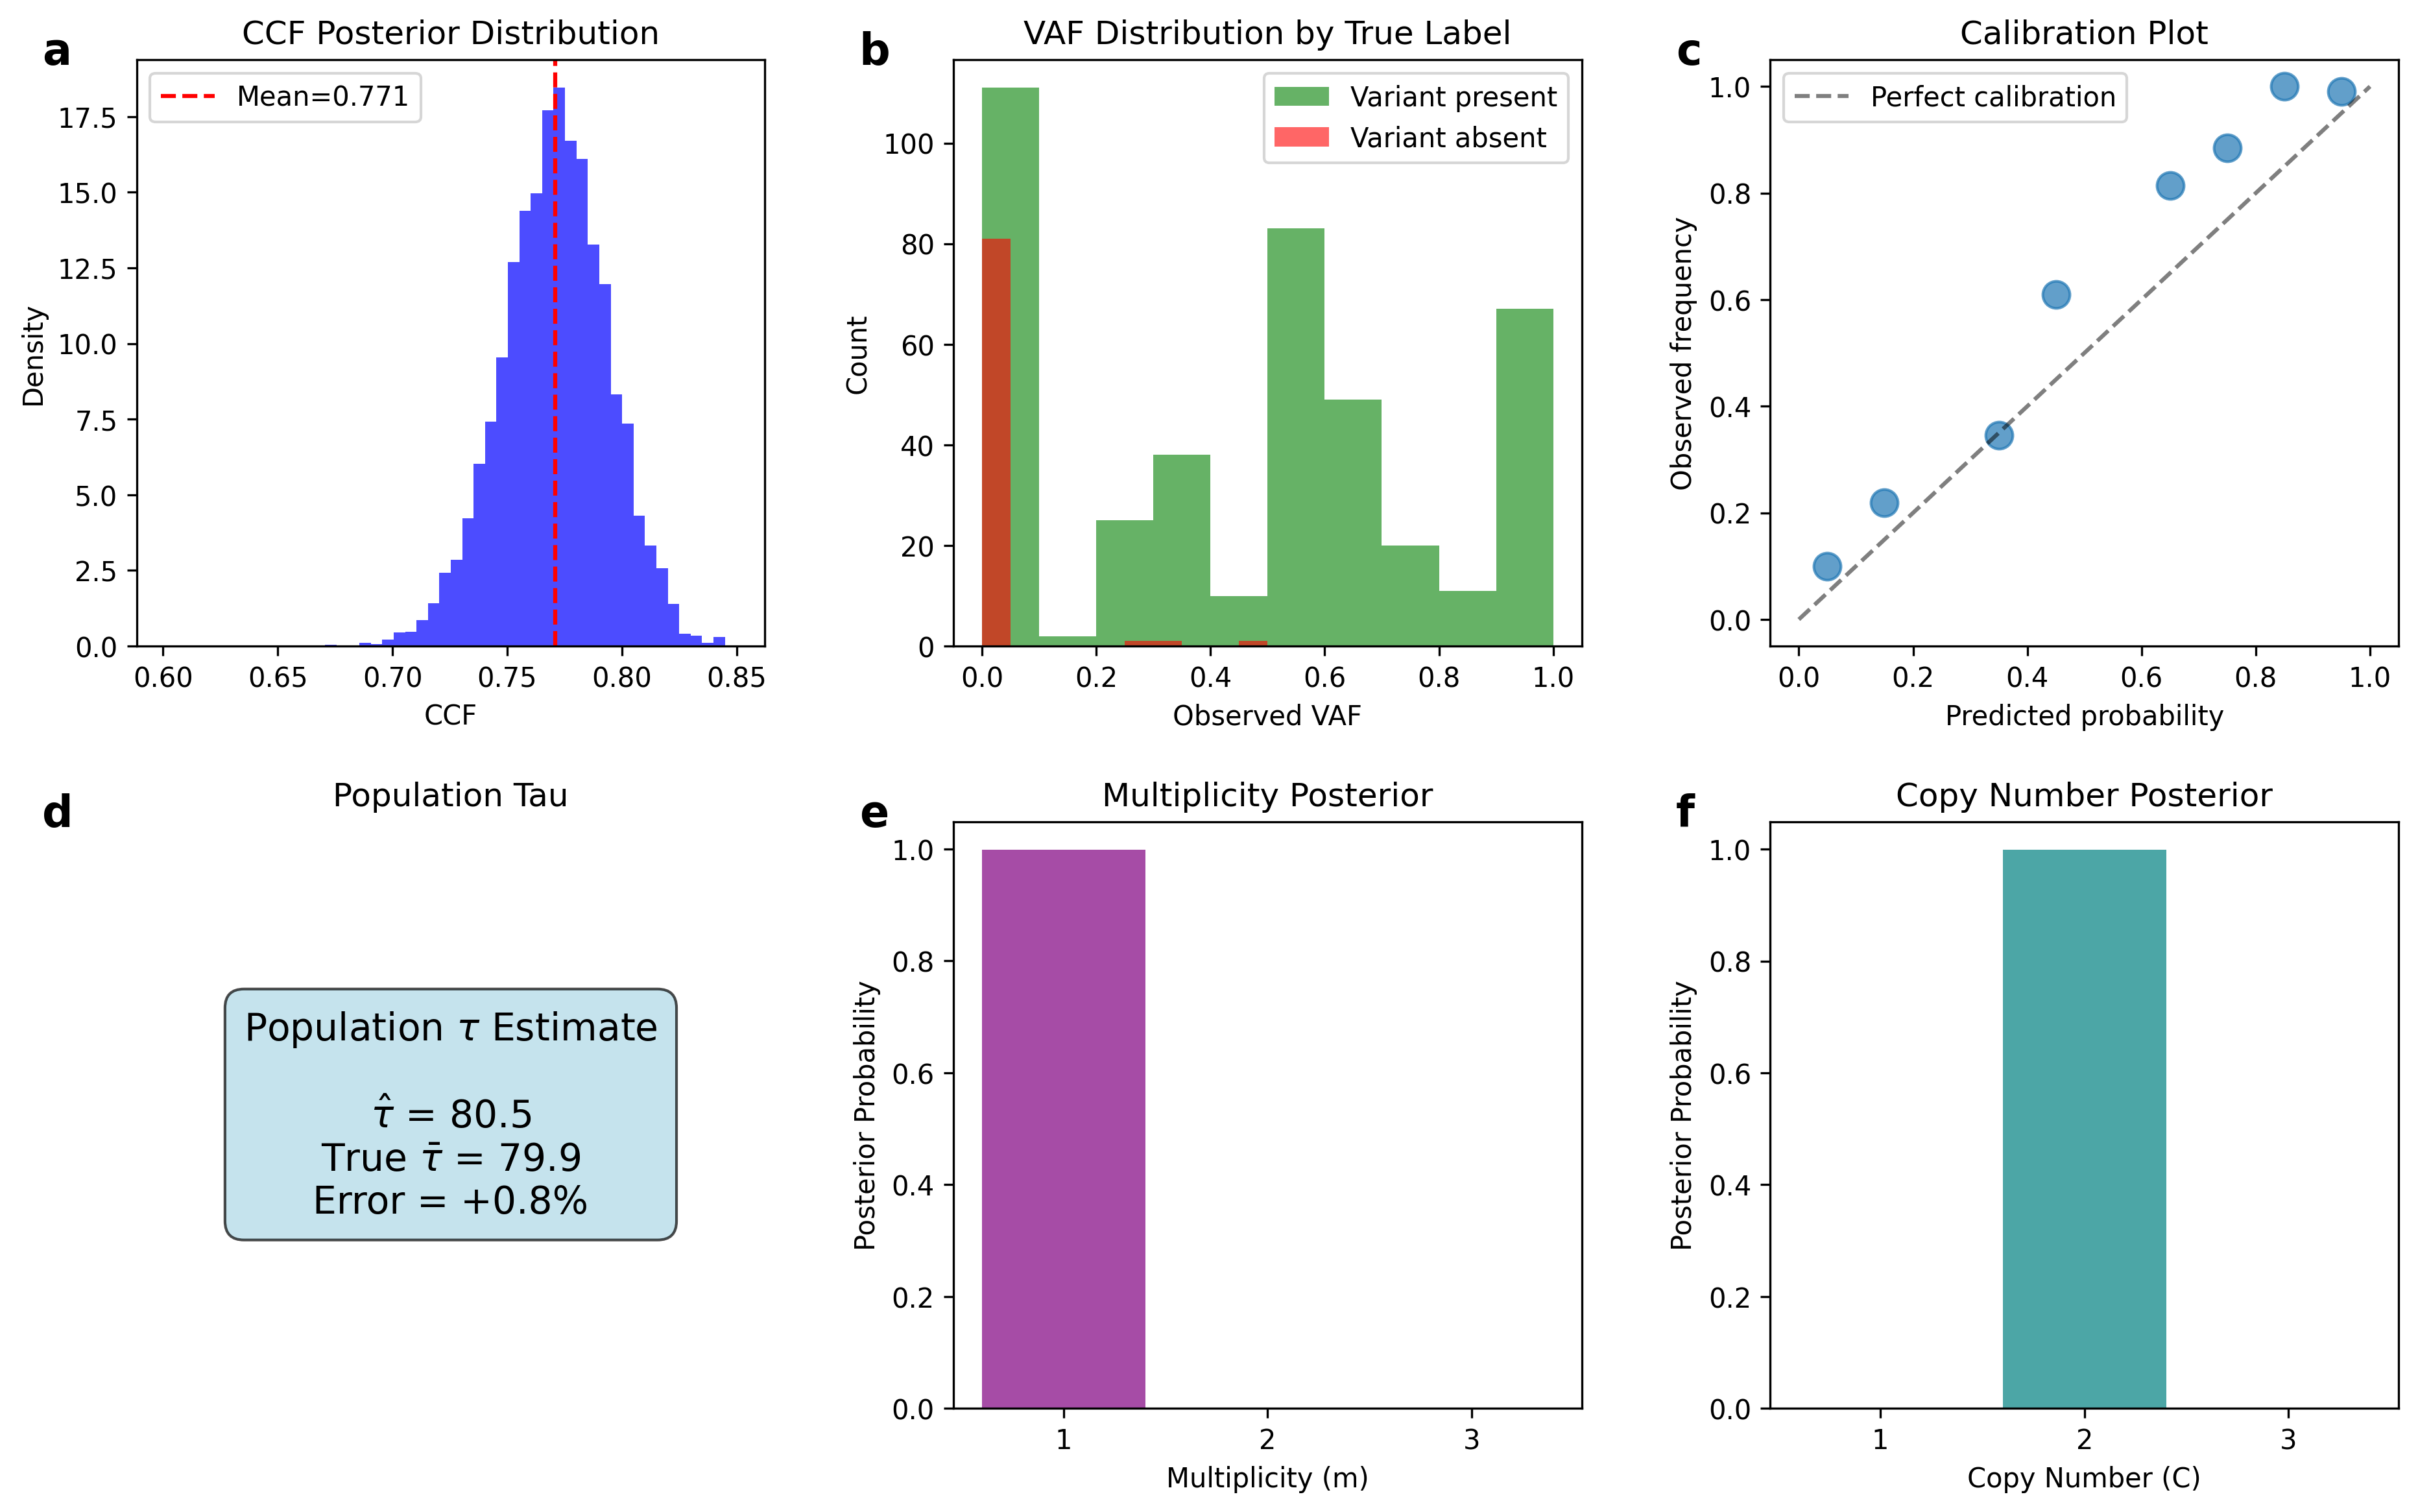
\includegraphics[width=\textwidth]{../data/almost_all_cells_positive/bayesian_plots_diagnostics.png}
    \caption{\textbf{High CCF diagnostics.} (a) CCF posterior distribution . (b) Observed VAF distribution by true variant status. (c) Calibration plot demonstrating well-calibrated posteriors: predicted probabilities accurately reflect observed frequencies. (d) MLE estimate of $\tau$, true $\tau$, and percentage error. (e) Multiplicity posterior. (f) Copy number posterior.}
    \label{fig:high-ccf-diagnostics}
\end{figure}

\subsection{Intermediate Prevalence}

Figure~\ref{fig:mid-ccf-results} shows results for the intermediate CCF scenario (approximately 250/500 cells harbor the variant). The same systematic posterior shift is visible (Figure~\ref{fig:mid-ccf-results}a), although attenuated compared to the high CCF case. Both methods achieve similar maximum F1 = 0.87, with optimal thresholds of 0.54 (Bayesian) and 0.17 (naive) (Figure~\ref{fig:mid-ccf-results}b). ROC-AUC is 0.937 for Bayesian versus 0.895 for naive. The CCF posterior (Figure~\ref{fig:mid-ccf-diagnostics}a) again recovers the true value, with mean 0.539 versus the simulation parameter of 0.50.

\begin{figure}[htbp]
    \centering
    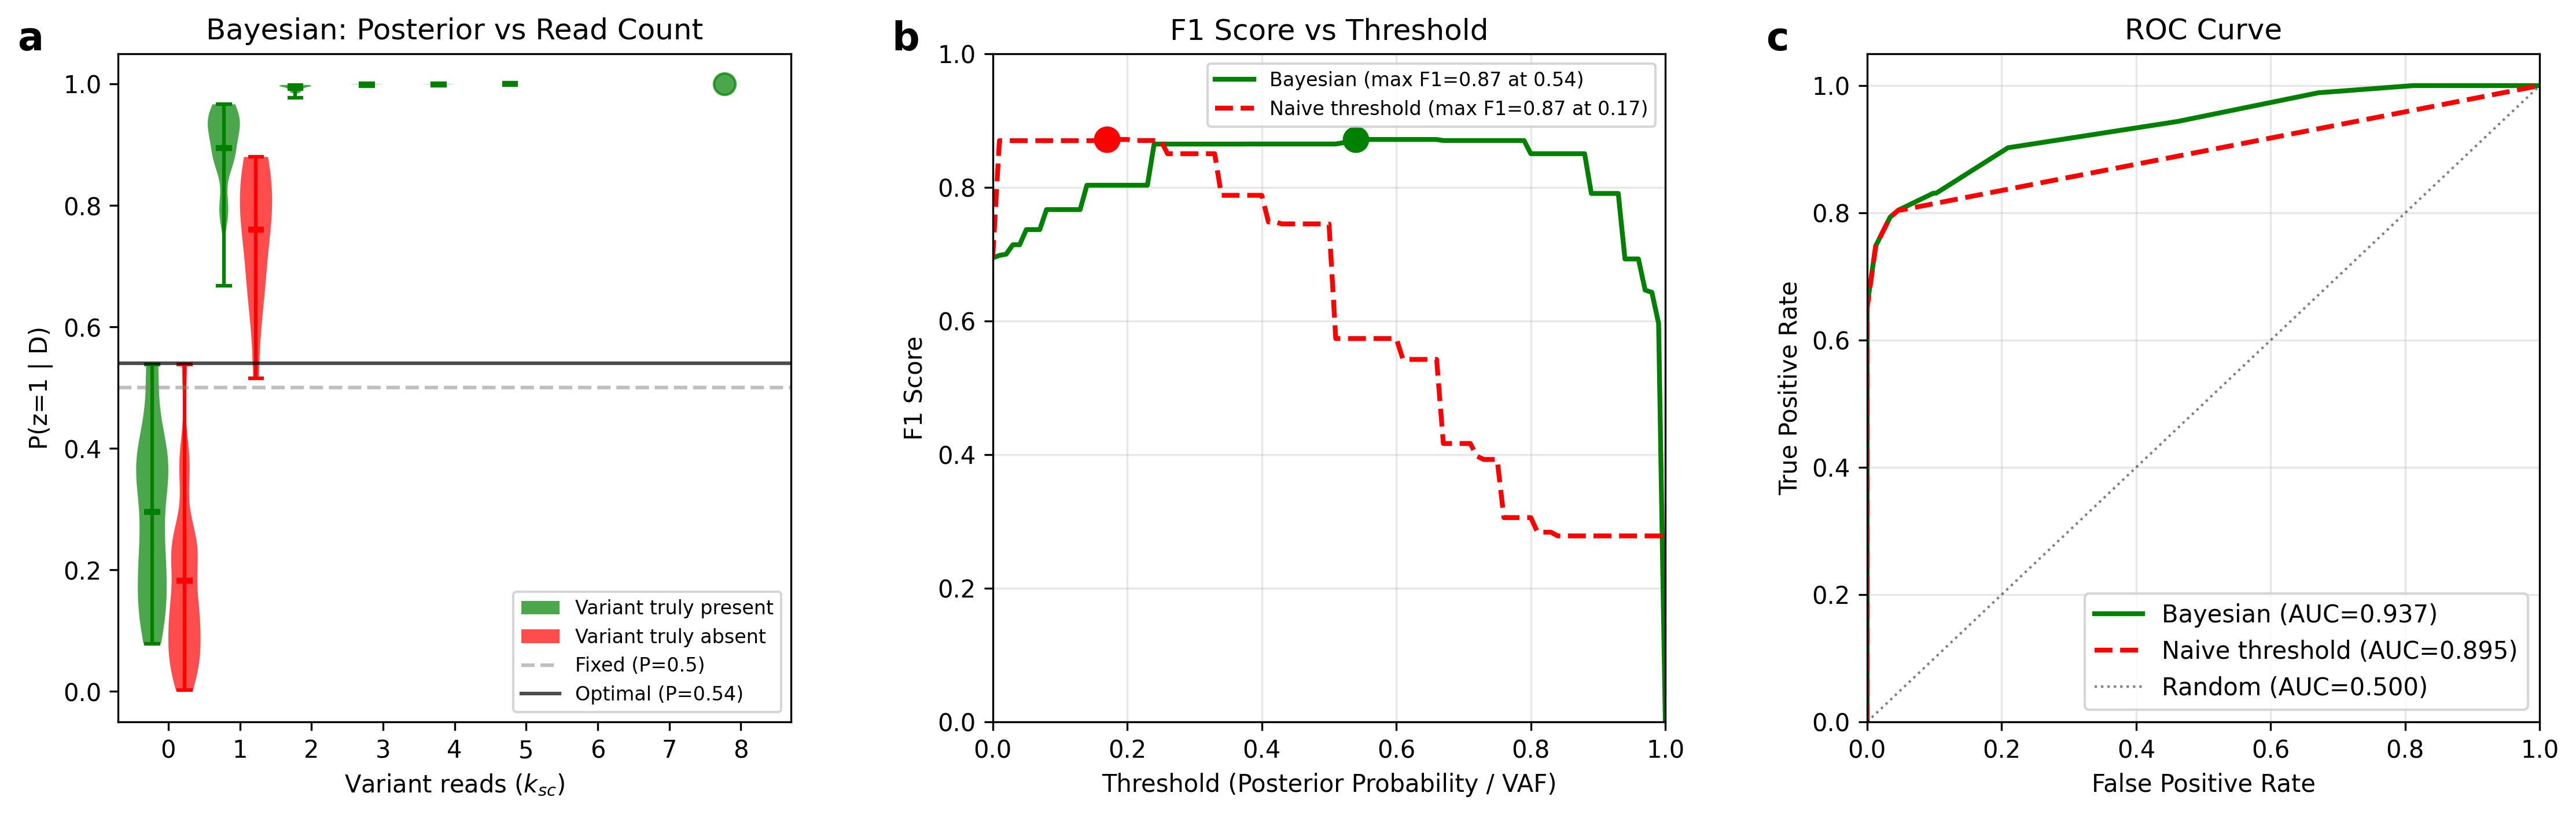
\includegraphics[width=\textwidth]{../data/half_half/bayesian_plots.png}
    \caption{\textbf{Intermediate CCF inference results (CCF = 0.5).} (a) Posterior probability versus $k_{sc}$. (b) F1-score versus threshold. (c) ROC curves for Bayesian and naive methods.}
    \label{fig:mid-ccf-results}
\end{figure}

\begin{figure}[htbp]
    \centering
    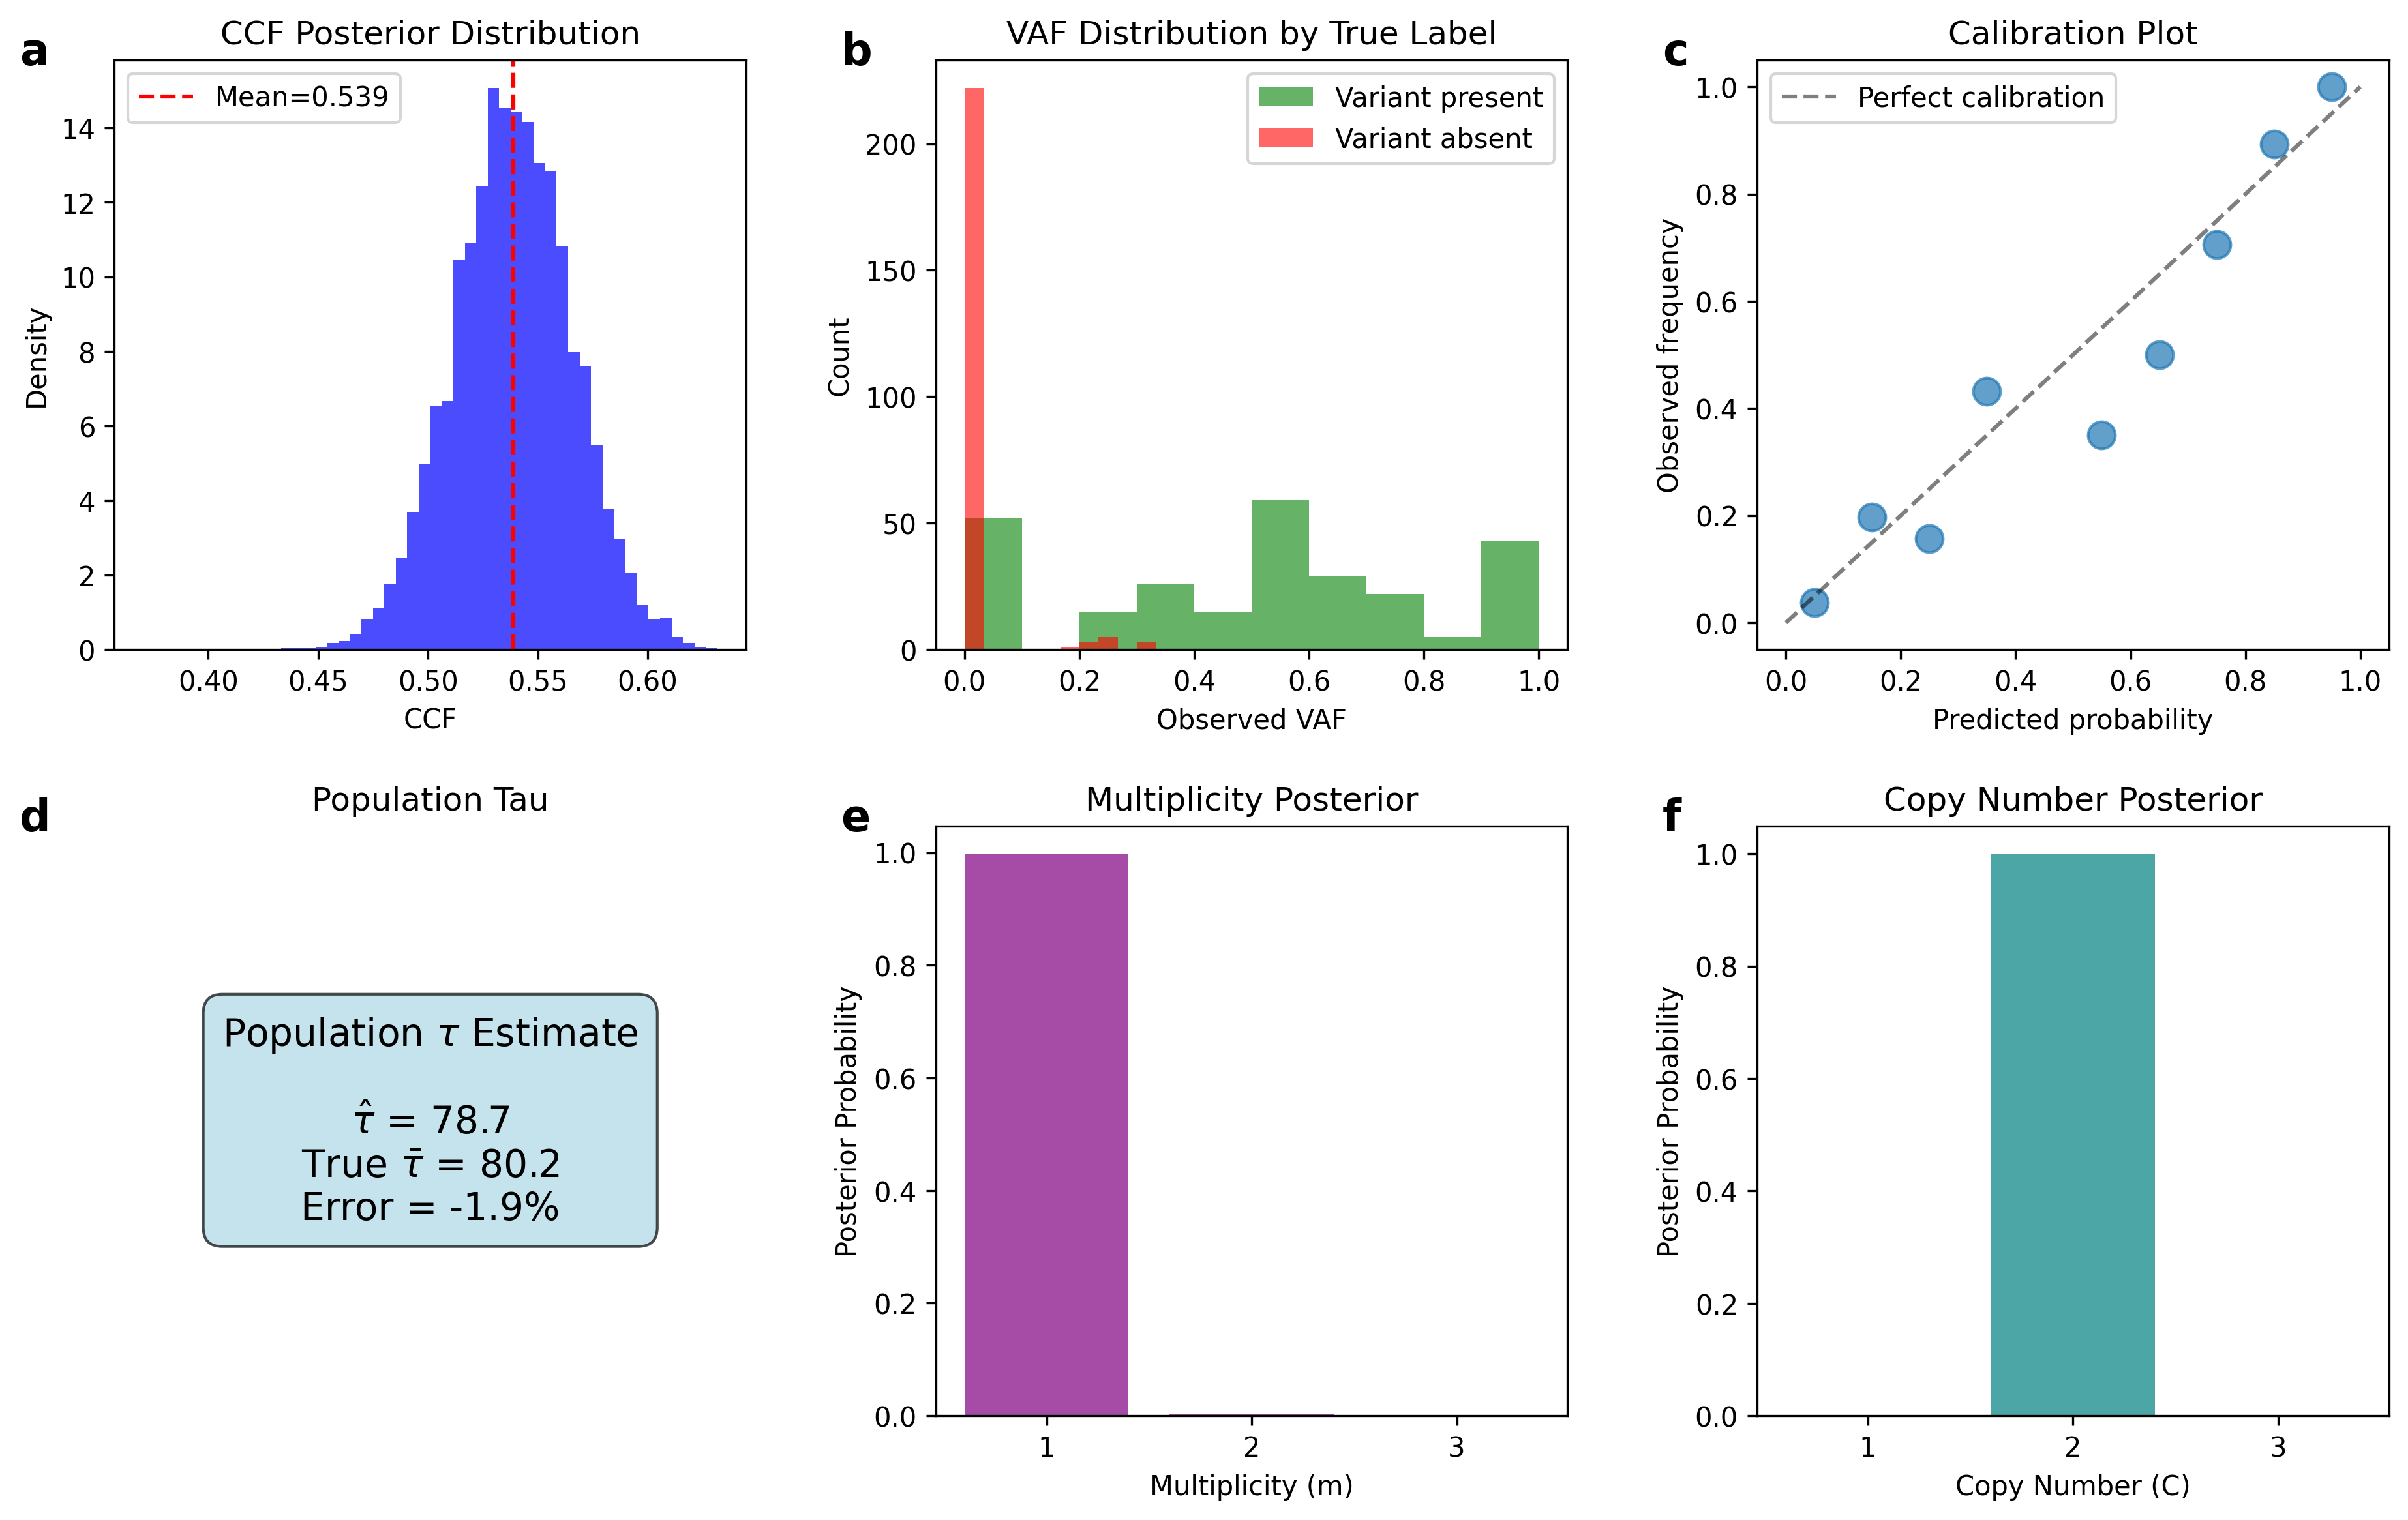
\includegraphics[width=\textwidth]{../data/half_half/bayesian_plots_diagnostics.png}
    \caption{\textbf{Intermediate CCF diagnostics.} (a) CCF posterior distribution (simulation parameter 0.50). (b) VAF distribution by true status. (c) Calibration plot. (d) MLE estimate of $\tau$, true $\tau$, and percentage error. (e) Multiplicity posterior. (f) Copy number posterior.}
    \label{fig:mid-ccf-diagnostics}
\end{figure}

\subsection{Low Prevalence}

Figure~\ref{fig:low-ccf-results} shows results for the low CCF scenario (approximately 100/500 cells harbor the variant). Dropout cells ($k_{sc}=0$) receive low posteriors consistent with the CCF prior, while cells with $k_{sc} \geq 1$ show strong upward shifts (Figure~\ref{fig:low-ccf-results}a). Both methods achieve maximum F1 = 0.80, with optimal thresholds of 0.39 (Bayesian) and 0.21 (naive) (Figure~\ref{fig:low-ccf-results}b). ROC-AUC is 0.946 for Bayesian versus 0.867 for naive. CCF, multiplicity, and copy number posteriors (Figure~\ref{fig:low-ccf-diagnostics}) accurately recover the ground truth.

\begin{figure}[htbp]
    \centering
    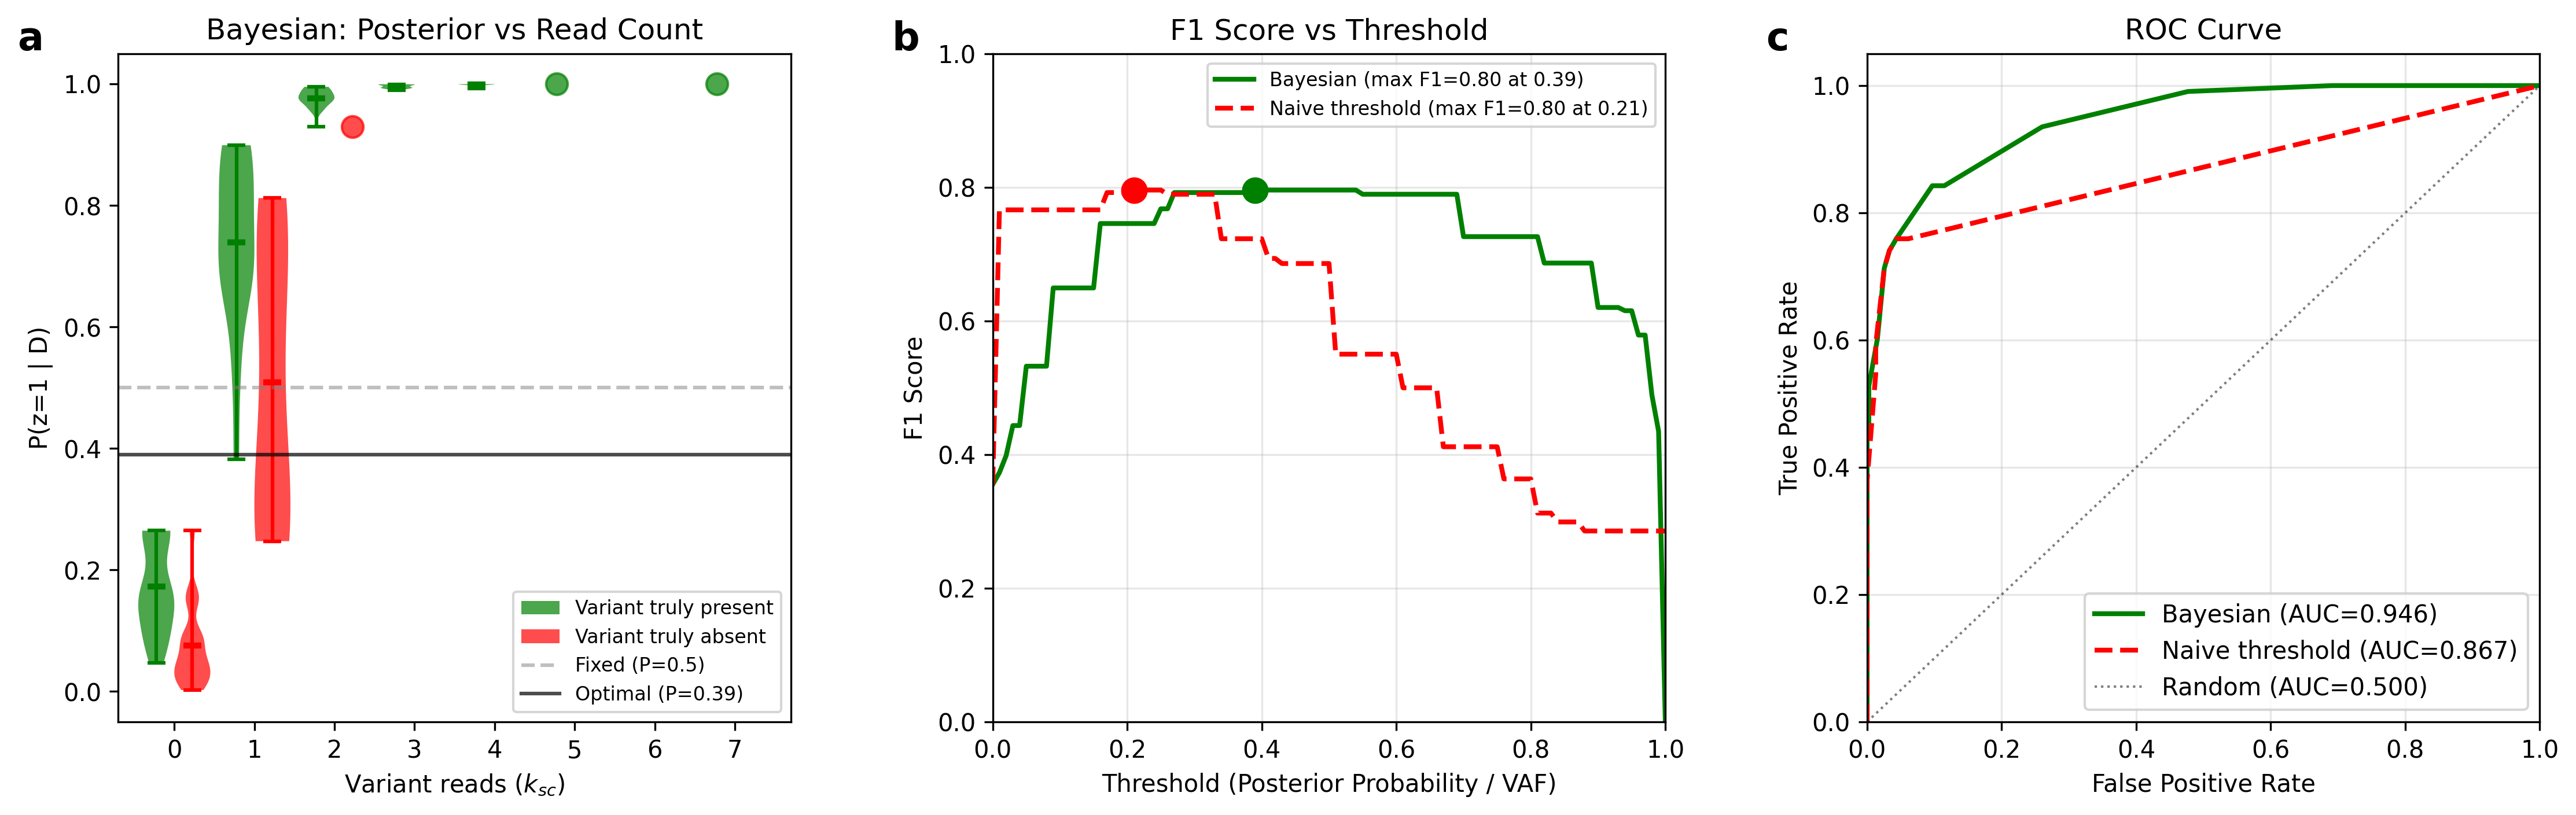
\includegraphics[width=\textwidth]{../data/almost_all_cells_negative/bayesian_plots.png}
    \caption{\textbf{Low CCF inference results (CCF = 0.2).} (a) Posterior probability versus $k_{sc}$. (b) F1-score versus threshold. (c) ROC curves.}
    \label{fig:low-ccf-results}
\end{figure}

\begin{figure}[htbp]
    \centering
    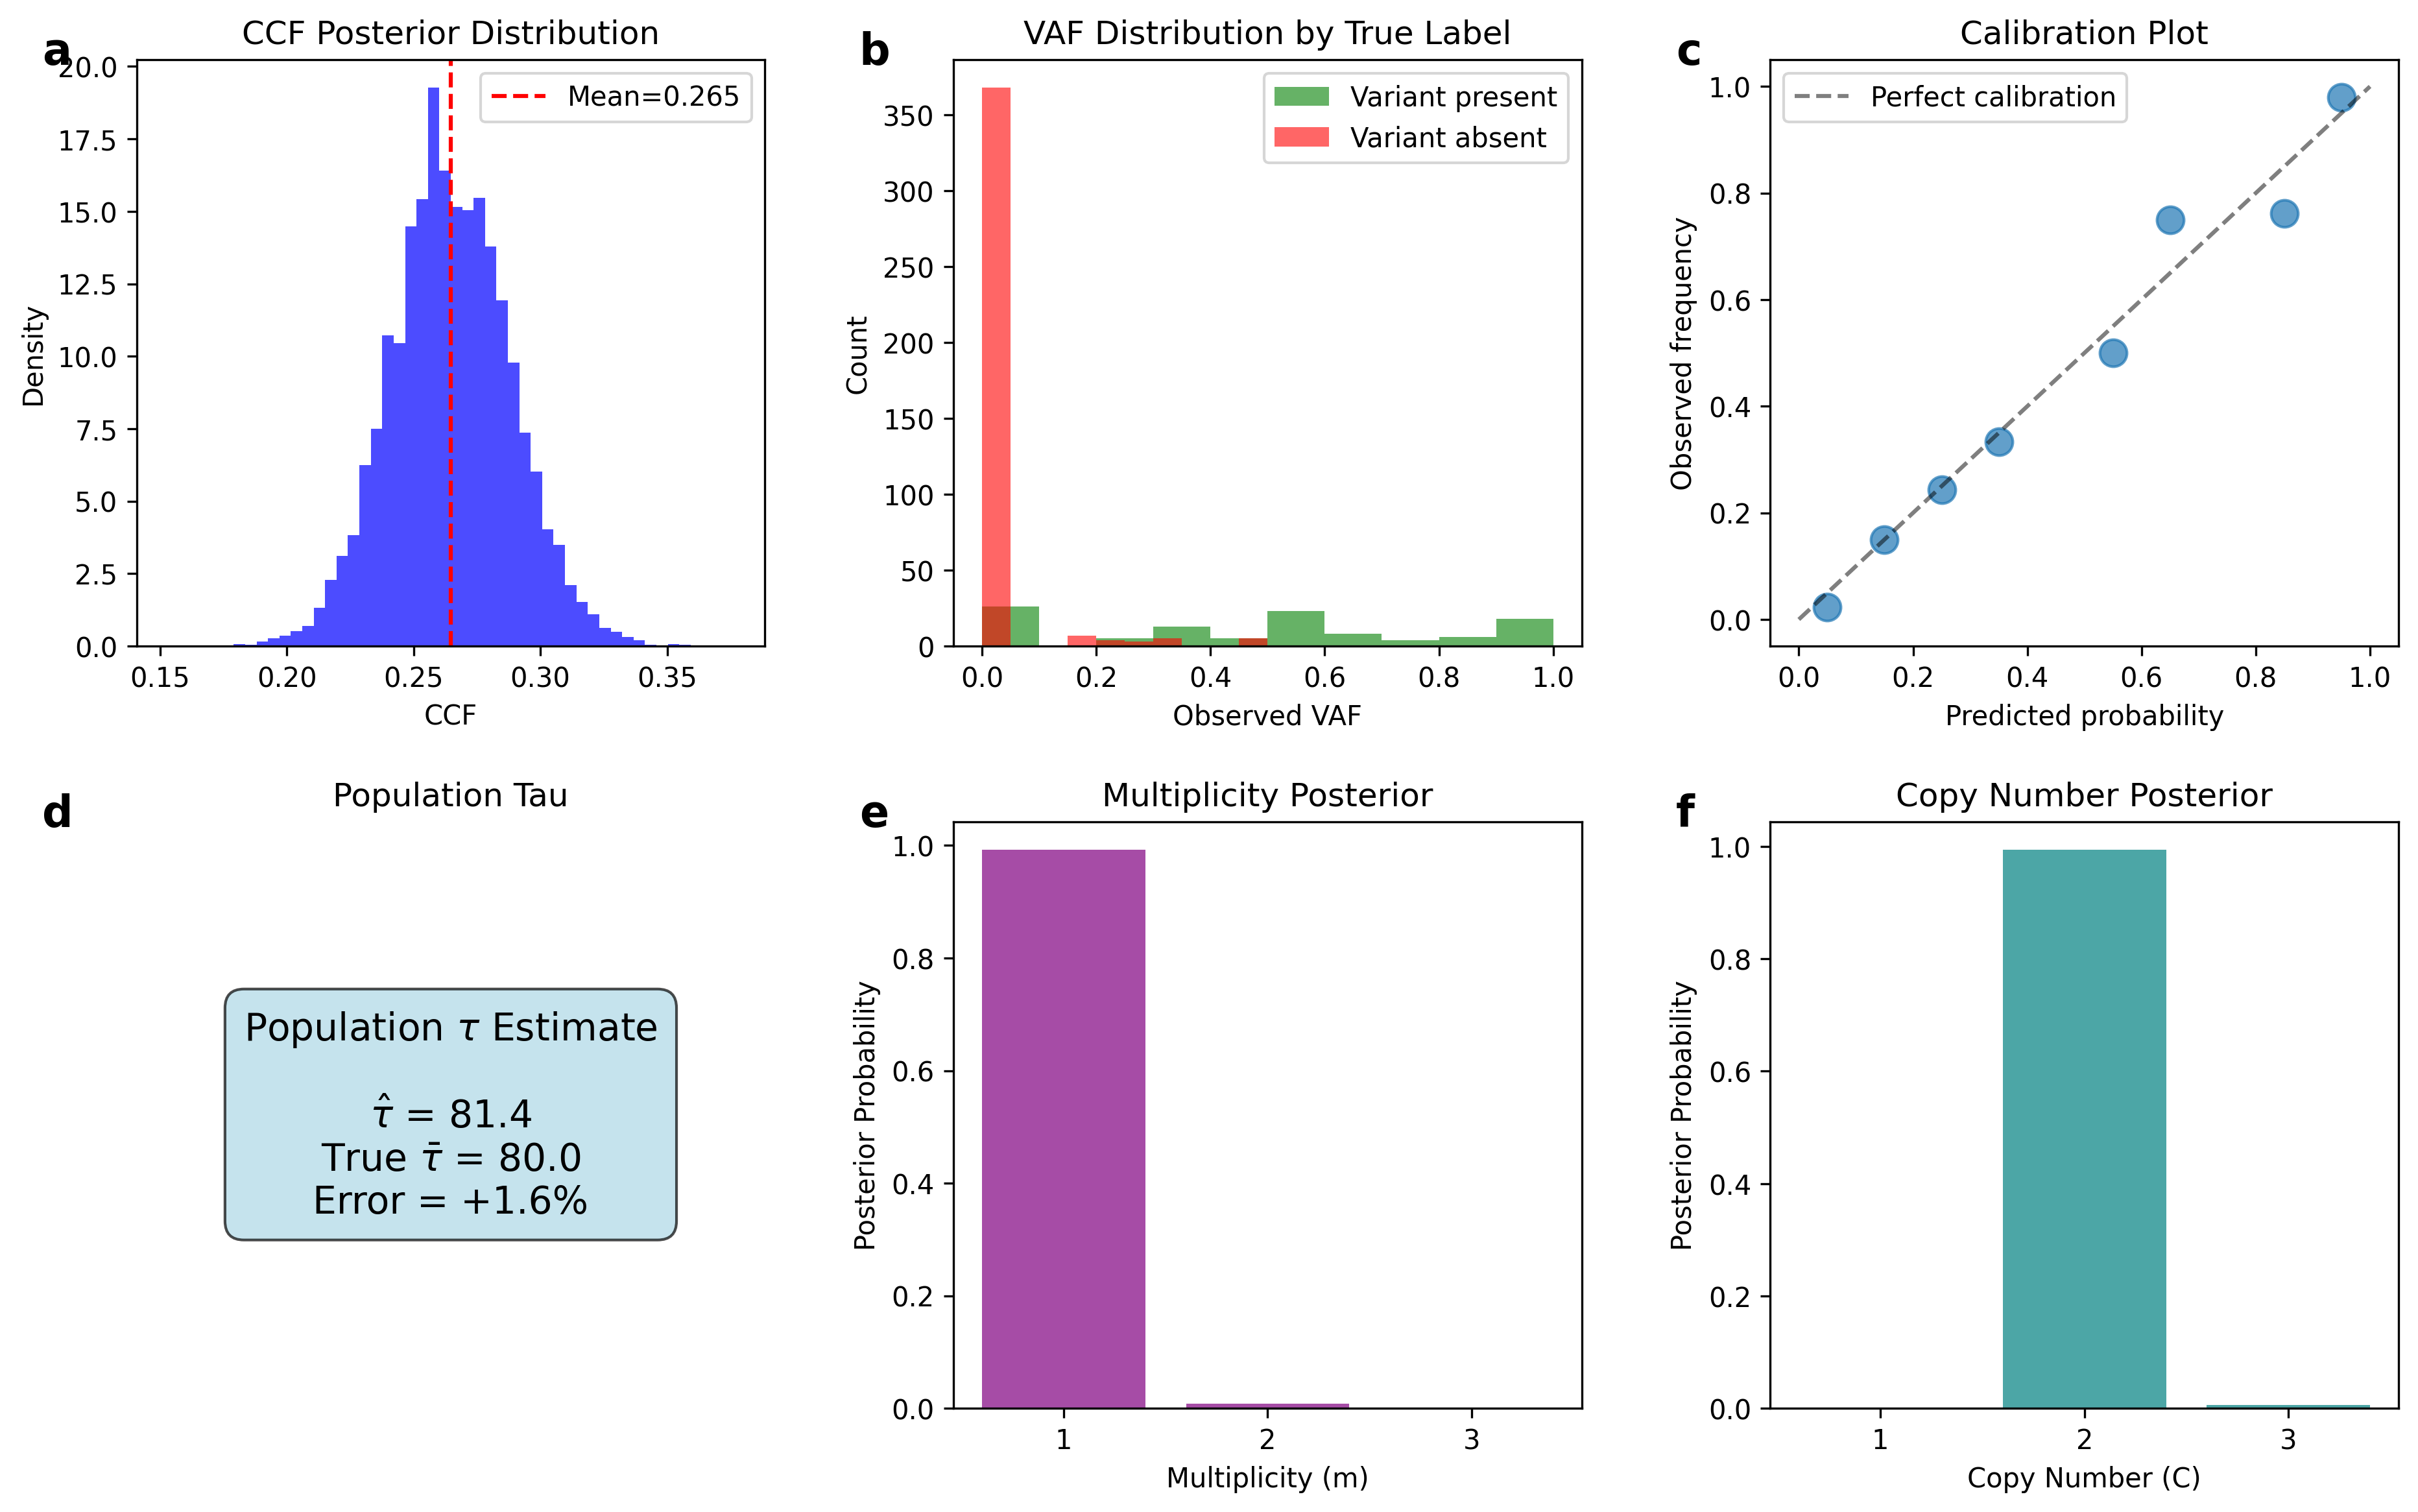
\includegraphics[width=\textwidth]{../data/almost_all_cells_negative/bayesian_plots_diagnostics.png}
    \caption{\textbf{Low CCF diagnostics.} (a) CCF posterior distribution (b) VAF distribution by true status. (c) Calibration plot. (d) MLE estimate of $\tau$, true $\tau$, and percentage error. (e) Multiplicity posterior. (f) Copy number posterior.}
    \label{fig:low-ccf-diagnostics}
\end{figure}

\section{Discussion}
\label{sec:discussion}

SC-BIG consistently achieves higher ROC-AUC than naive thresholding across all CCF regimes (0.934--0.946 vs.\ 0.857--0.895), indicating superior discrimination independent of threshold choice. Maximum F1 scores are nearly identical between methods. However, this apparent parity masks the fact that naive thresholding requires knowing the optimal threshold a priori---which is impossible in practice---while SC-BIG's calibrated posteriors enable threshold selection based on application-specific precision-recall trade-offs. The naive method's F1 curve tends to peak sharply at a specific threshold and degrade away from this optimum. This effect is most pronounced at high CCF (Figure~\ref{fig:high-ccf-results}b). SC-BIG on the other hand maintains high F1 across a broader threshold range.

$P(z=1|D)$ distributions reveal SC-BIG's core advantage: at every $k_{sc}$ value, variant-present cells consistently receive higher posteriors on average than variant-absent cells. This systematic upward shift in the posterior distribution---not just at the decision boundary but across the entire range---reflects the model's effective integration of bulk-derived CCF information with single-cell observations. Even for $k_{sc}=0$, where both cell types produce identical read evidence, the posterior distributions separate based on the CCF prior.

At high CCF (0.8), SC-BIG achieves a 3-point improvement in maximum F1 (0.94 vs.\ 0.91). When 80\% of cells harbor the variant, even dropout cells receive elevated posteriors driven by the CCF prior, allowing recovery of true positives that naive thresholding necessarily misses.

At intermediate and low CCF (0.5 and 0.2), both methods achieve similar maximum F1 (0.87 and 0.80 respectively). This convergence is expected: when the CCF prior is near or below 0.5, dropout cells correctly receive low posteriors, and the classification problem reduces to distinguishing cells with $k_{sc} \geq 1$. However, the ROC-AUC gap remains substantial (4--8 percentage points), indicating that SC-BIG provides better ranking even when optimal F1 is matched. Notably, these results were obtained with a relatively wide prior on copy number ($\sigma_C = 0.3$), demonstrating robustness to uncertainty in this input parameter.

CCF posterior estimates exhibit moderate bias in two directions: at high CCF, allelic dropout causes the empirical CCF prior to undercount variant-positive cells, pulling the posterior downward; at low CCF, sequencing errors ($\epsilon_{sc}$) cause variant-absent cells to produce spurious variant reads ($k_{sc} \geq 1$), inflating the empirical prior and biasing the posterior upward. Both effects are small relative to the posterior width and do most likely not affect genotyping accuracy.

Beyond improved classification metrics, SC-BIG provides interpretable uncertainty quantification through well-calibrated posterior probabilities. The method outputs a matrix of genotype probabilities that quantifies confidence in variant presence. Calibration plots (Figures~\ref{fig:high-ccf-diagnostics}c, \ref{fig:mid-ccf-diagnostics}c, \ref{fig:low-ccf-diagnostics}c) demonstrate that across all CCF regimes, a cell assigned posterior probability $p$ truly harbors the variant with frequency $\approx p$. This calibration enables principled decision-making: researchers can select thresholds based on their tolerance for false positives versus false negatives, with transparent interpretation of the trade-offs. Additionally, calibrated posteriors enable direct integration into downstream probabilistic analyses. Phylogenetic reconstruction methods such as CellPhy~\cite{kozlov2022} can incorporate genotyping uncertainty via genotype likelihoods as input, yielding more accurate trees than methods that require binary genotype calls. Similarly, clonal structure inference can propagate uncertainty from variant calls through to clonal assignments.

The presented work is limited in several ways. Our evaluation focused on three CCF values with fixed biological parameters. A systematic grid search varying purity, copy number, multiplicity, coverage, and error rates would characterize performance across the full parameter space and identify conditions where the Bayesian approach provides the greatest benefit. Furthermore, per-cell copy number estimates can readily be obtained from scDNA-seq. Incorporating these as informative priors on $C$ (rather than using bulk-derived estimates) could substantially improve inference, particularly for aneuploid tumors where copy number varies across cells. To further improve model performance, future work will incorporate phylogenetic constraints, for example the requirement that mutations appearing in a distinct subclone also appear in ancestral cells. Lastly, we are currently applying SC-BIG to an existing cohort with paired single-cell and bulk sequencing data. Real data validation is essential as it introduces systematic biases (GC content, mappability) and model violations that simulations cannot capture. Datasets with orthogonal truth would enable rigorous benchmarking against existing single-cell genotyping software.

\section{Acknowledgements}

\noindent DS is partially funded through a research grant by the E.I. Stiftung Kölner Krebsforschung. RFS is a Professor at the Cancer Research Center Cologne Essen (CCCE) funded by the Ministry of Culture and Science of the State of North Rhine-Westphalia. The authors thank the Regional Computing Center of the University of Cologne (RRZK) for providing computing time on the High Performance Computing (HPC) system RAMSES as well as support. The large language model Claude was used for proof-reading and improving the clarity of the manuscript.~\cite{claude3}

\pagebreak

\section{Bibliography}

\printbibliography[heading=none]

\end{document}
